\chapter{Energia}
Fino a questo punto, in tutti gli esercizi, abbiamo fatto largo uso del tempo per poter calcolare ciò che ci richiedeva il problema.
Questo approccio, però, è molto limitato perché le forze in generale non sono costanti nel tempo, ma sono costanti nello spazio \label{costantiSpazio}, come vedrete a seguito nella spiegazione di lavoro di una forza costante e variabile.

Essendo l’energia ovunque, sotto diverse forme, l'energia di un corpo, o sistema, è possibile trovarla prima che il moto succeda.

\section{Che cos'è l'energia? }
L’energia, in fisica, è una grandezza che esprime la capacità di un corpo, o di un sistema, di compiere un lavoro, ed è associata ad una grandezza scalare: il Joule $[J = Nm]$
\paragraph{}
Ci sono diversi tipi di energia, in particolare a noi ne interessano tre:

\begin{itemize}
    \item Energia cinetica $E_c$
    \item Energia potenziale $E_p$
    \item Energia meccanica $E_{tot}$
\end{itemize}

Dove l’energia meccanica è definita come la somma di energia cinetica e di energia potenziale dello stesso sistema. 

\newpage
\subsection{Il lavoro compiuto da una forza costante}

\begin{figure}[tb]
    \centering
    \begin{tikzpicture}[scale = 1.3]
      \def\ul{0.52}
      \def\R{3.1}
      \def\ang{26}
      \coordinate (O) at (0,0);
      \coordinate (R) at (\ang:\R);
      \coordinate (X) at ({\R*cos(\ang)},0);
      \draw[projcol,dashed] (R) -- (X);
      \draw[vector] (O) -- (R) node[midway,left=5,above right=0] {$\vec{A}$};
      \draw[vector,projcol]
        (O) -- (X) node[scale=0.8,left=4,below=-1] {$\vec{A}\text{x}\vec{B} = AB\cos\theta$};
      \draw[vector,unitcol]
        (O) -- (\ul,0) node[scale=0.9,left=2,below left=0] {$\vec{B}$};
      \draw pic[->,thick,"$\theta$",draw=black,angle radius=26,angle eccentricity=1.3]
        {angle = X--O--R};
    \end{tikzpicture}
    \caption{Prodotto Scalare}
    \label{fig:prodScalare}
\end{figure}

Per svolgere i calcoli rispolveriamo il concetto di prodotto scalare tra due vettori:

\begin{equation*}
    \vec{A}\cdot \vec{B} = AB\cos\theta
\end{equation*}

Il risultato è uno scalare, un numero, che rappresenta la proiezione del vettore $\vec{A}$ sul vettore $\vec{B}$ come è raffigurato nella Figura \ref{fig:prodScalare}.

Data una forza costante $\vec{F}$ esercitata su un corpo che effettua uno spostamento rettilineo $\vec{s}$, possiamo scrivere la formula del lavoro:

\begin{equation*}
    L = \vec{F} \cdot \vec{s}
\end{equation*}

Essendo che la forza e lo spostamento sono vettori, il prodotto della formula precedente è un prodotto scalare e dunque possiamo scrivere equivalentemente:

\begin{equation}
    L = Fs\cos\theta
    \label{lavoroForzaConst}
\end{equation}

\begin{figure}[H]
    \centering
    
    \begin{tikzpicture}[scale = 1.3]
      \def\W{2.7}  % ground width
      \def\D{0.2}  % ground depth
      \def\h{0.8}  % mass height
      \def\w{1.0}  % mass width
      \def\F{1.1}  % force magnitude
      \def\ang{30} % angle force
      \coordinate (F0) at (0.4*\w,0.85*\h);
      \coordinate (Fx) at ($(F0)+({\F*cos(\ang)},0)$);
      \coordinate (F)  at ($(F0)+(\ang:\F)$);
      \draw[ground] (-0.3*\W,0) rectangle++ (\W,-\D);
      \draw (-0.3*\W,0) --++ (\W,0);
      \draw[mass] (-\w/2,0) rectangle++ (\w,\h) node[midway] {$m$};
      \draw[force,xcol] (\w/2,0.15*\h) --++ (0.4*\W,0) node[midway,above=-1.5] {$\vb*{s}$};
      \draw[dashed,myred!80!black!60] (Fx) -- (F);
      \draw[Fproj] (F0) -- (Fx) node[above=1,right=-1] {$F\cos\theta$}; %\vu{x}
      \draw[force] (F0) -- (F)  node[above=1,right=-1] {$\vec{F}$};
      \draw pic["$\theta$",draw=black,angle radius=14,angle eccentricity=1.4] {angle=Fx--F0--F};
    \end{tikzpicture}
    \caption{Lavoro di un corpo sottoposto ad una forza $\vec{F}$}
    \label{fig:lavoroCorpoSottopostoForza}
\end{figure}

\subsection{Il lavoro compiuto da una forza variabile}

Per introdurre la nozione di lavoro compiuto da una forza variabile consideriamo uno spostamento unidirezionale lungo l’asse X e la forza F in funzione dello spostamento. 

Immaginiamo ora di suddividere lo spostamento in tanti piccoli intervalli in modo da considerare la forza costante in ciascuno di essi. Figura \ref{lavoro}.
\paragraph{}
Dunque il lavoro totale sarà la forza di ogni lavoro constante in ciascun intervallo: 

\begin{equation*}
    L \simeq \Delta L_1 + \Delta L_2 + \dots +  \Delta L_n = F_1\Delta_x + F_2\Delta_x + \dots + F_n\Delta_x
\end{equation*}
\begin{equation}
    L \simeq \sum_{k = 1} ^ n F_k \Delta_x
\end{equation}


Siccome vogliamo calcolare precisamente il lavoro, dobbiamo far tendere a zero l'intervallo $\Delta_x$. Per ottenere il risultato voluto utilizziamo la nozione di limite:
\begin{equation}
    L = \lim_{\Delta_x \to 0} \sum_{k = 1} ^ n F_k \Delta_x
    \label{limiteIntervalloInfinitesimoLavoro}
\end{equation}

Questa formula altro non è che:

\begin{equation}
    L = \int_{x_1}^{x_2} F(x) \, dx = E_{(p_2)} - E_{(p_1)}
\end{equation}

Svolgendo i calcoli si ottiene che:
\begin{equation*}
    L = \int_{x_1}^{x_2} F(x) \, dx = F[x]_{x_1}^{x_2} = F(x_2 - x_1) = Fs
\end{equation*}

La differenza tra posizione finale e posizione iniziale è proprio uguale allo spostamento e dunque ci siamo ricondotti alla formula del lavoro di una forza costante: \ref{lavoroForzaConst}.

Tutto questo per spiegare perché a Pagina~\pageref{costantiSpazio} ho affermato che: "le forze in generale non sono costanti nel tempo, ma sono
costanti nello spazio".


\begin{figure}[tb]
    \centering
    % WORK diagram - curve
\def\xmax{3.4}
\def\ymax{2.2}
\begin{tikzpicture}[scale = 1.3]
  \def\x{.58*\xmax}
  \def\dx{.07*\xmax}
  \def\F{.75*\ymax}
  
  % AREA
  \coordinate (Ax) at (.12*\xmax,0);
  \coordinate (Cx) at (.84*\xmax,0);
  \coordinate (A) at (.12*\xmax,.55*\ymax);
  \coordinate (B) at (.48*\xmax,.80*\ymax);
  \coordinate (C) at (.84*\xmax,.60*\ymax);
  \fill[xcol!20] (A) to[out=10,in=180] (B) to[out=0,in=170] (C) |- (Ax) -- cycle;
  \path (Ax) -- (C) node[midway,left=-2,blue] {$L$};
  
  % LINE
  \draw[very thick,xcol] (A) to[out=10,in=180] (B) to[out=0,in=170] (C);
  \fill[xcol] (A) circle (0.04); %node[right=5,above=2] {$P_1$, $V_1$};
  \fill[xcol] (C) circle (0.04); %node[right=2] {$P_2$, $V_2$};
  
  % AXIS
  \draw[->,thick] (0,-0.1*\ymax) -- (0,\ymax); %node[left] {$F$};
  \draw[->,thick] (-0.1*\xmax,0) -- (\xmax,0) node[below] {$x$};
  \tick{Ax}{90} node[below] {$x_1$};
  \tick{Cx}{90} node[below] {$x_2$};
  \tick{0,\F}{0} node[left] {$F$};
  
  % RECTANGLE
  \draw[dashed] (0,\F) --++ (\x,0);
  \draw[xcol] (\x,0) rectangle++ (\dx,\F);
  \draw[smallarrow] (\x,-0.08) --++ (\dx,0) node[midway,below=0,scale=0.9] {$\Delta{x}$};
  %\node[below=-1] at (\x+\dx/2,0) {$\Delta x$};
  
\end{tikzpicture}
    \caption{Significato geometrico del lavoro}
    \label{lavoro}
\end{figure}

\subsection[Espressione generica del lavoro]{Espressione generica del lavoro con forze costanti e traiettoria qualsiasi}

\begin{figure}[H]
    \centering
    % CURVED PATH
    \begin{tikzpicture}
      \def\ul{0.6}
      \def\Ra{1.4}
      \def\Rb{0.8}
      \def\anga{0}
      \def\angb{25}
      \coordinate (A) at (0,0);
      \coordinate (B) at (1.1,1.9);
      \coordinate (C) at (2.1,1.0);
      \coordinate (D) at (3.7,0.4);
      \coordinate (E) at (5.1,2.1);
      
      \draw[xcol,thick]
        (A)++(-140:0.4) to[out=20,in=-120]
        (A) to[out=60,in=\anga-180]
        (B) to[out=\anga,in=100]
        (C) to[out=-80,in=\angb-180]
        (D) to[out=\angb,in=-120]
        (E) to[out=60,in=-160]++ (40:0.4);
      
      % PATH DIFFERENCE
      \draw[vector,acol]
        (B) --++ (\anga:0.5) coordinate (BS) node[above=2,right=-2] {$\vec{\dd r}$};
      \draw[vector,acol]
        (D) --++ (\angb:0.5) coordinate (DS) node[below right=-4] {$\vec{\dd r}$}; %above left=-4
      
      % FORCE
      \draw[force]
        (B) --++ (-80:0.8) coordinate (BF) node[below=-1] {$\vec{F}$};
      \draw[force]
        (D) --++ (145:0.6) coordinate (DF) node[above left=-3] {$\vec{F}$};
      \draw pic["$\theta$",draw=black,angle radius=6,angle eccentricity=1.8] {angle=BF--B--BS};
      \draw pic["$\theta$",draw=black,angle radius=6,angle eccentricity=1.8] {angle=DS--D--DF};
      
      \fill[xcol] (A) circle (2pt) node[above left=-1] {$A$};
      %\fill[xcol] (B) circle (2pt);
      %\fill[xcol] (C) circle (2pt);
      %\fill[xcol] (D) circle (2pt);
      \fill[xcol] (E) circle (2pt) node[below right=-1] {$B$};
      
    \end{tikzpicture}
    \caption{Lavoro di una forza variabile lungo una traiettoria qualsiasi}
    \label{fig:lavoroForzaVariabileLunoTraiettQualsiasi}
\end{figure}

Sappiamo che:
\begin{equation*}
    \vec{F} \cdot \vec{dr} = \text{Lavoro infinitesimo}
\end{equation*}

Per ottenere quindi il lavoro che farà un oggetto che si sposterà dal punto A al punto B nella Figura \ref{fig:lavoroForzaVariabileLunoTraiettQualsiasi} dobbiamo calcolare: 

\begin{equation}
    L = \int_{A}^{B} \vec{F} \cdot \vec{dr} = \int_{A}^{B} F \cos\theta \, dr \quad [J = Nm]
    \label{formulaGeneraleLavoro}
\end{equation}

\section{Energia Cinetica}
L'energia cinetica è una forma di energia legata al movimento dei corpi nello spazio, in particolare alla loro massa e alla loro velocità.
Per calcolare l'energia cinetica in un sistema si utilizza la seguente formula:

\begin{equation}
    E_c = \frac{1}{2}mv^2\quad  [J = Nm]
    \label{energiaCinetica}
\end{equation}
e le relative formule inverse: 
\begin{equation}
    m = \frac{2E_c}{v^2} \quad  [Kg]\qquad v = \sqrt{\frac{2E_c}{m}} \quad  \biggl[\frac{m}{s}\biggl]
\end{equation}

\subsection{Teorema delle forze vive}

La formula \ref{energiaCinetica} deriva dalla seguente dimostrazione del teorema chiamato \textit{Teorema delle forze vive} o \textit{Teorema dell'energia cinetica}.
\paragraph{}
Partiamo dalla definizione di lavoro utilizzando la seconda legge di Newton \ref{secondaLeggeNewton}: 

\begin{equation*}
    L = \vec{F}\cdot s = m\veca \cdot \vec{s}
\end{equation*}

Questa equazione può essere scritta sotto forma di spostamenti infinitesimi ($\vec{dr}$)

\begin{equation*}
   \vec{F}\cdot\vec{dr} = m\frac{d\vec{v}}{d\vec{t}}\cdot d\vec{r}
\end{equation*}

Osserviamo che $\frac{\vec{dr}}{\vec{dt}}$, uno spostamento infinitesimo su un tempo infinitesimo, corrisponde alla definizione di velocità $\vec{v}$ quindi  che il lavoro elementare è:
\begin{equation*}
    \vec{F}\cdot\vec{dr} = md\vec{v}\cdot \vec{v}
\end{equation*}

Per l'espressione generica del lavoro con forze costanti e traiettoria qualsiasi, possiamo definire il lavoro come la somma di tutti gli spostamenti inifinitesimi, da $A$ a $B$ 

\begin{equation*}
     \int_{A}^{B} \vec{F} \cdot \vec{dr} = \int_{v_i}^{v_f} md\vec{v}\cdot \vec{v}
\end{equation*}

\begin{equation*}
    = E_{(p_2)} - E_{(p_1)} = m \biggl[\frac{v^2}{2}\biggl]_{v_i}^{v_f}
\end{equation*}

\begin{equation*}
    = E_{(p_2)} - E_{(p_1)} = \frac{1}{2}mv_f^2 - \frac{1}{2}mv_i^2
\end{equation*}
\begin{equation}
    = \frac{1}{2}mv_i^2 + E_{(p_2)}  =  \frac{1}{2}mv_f^2 + E_{(p_1)}
\end{equation}

Questa risoluzione è vera se e solo se siamo in presenza di forze conservative, e quindi abbiamo che il lavoro è indipendente dal percorso ma dipende solo dallo spazio effettivamente percorso. Figura \ref{fig:lavoroCostante}.

\begin{figure}[tb]
    \centering
    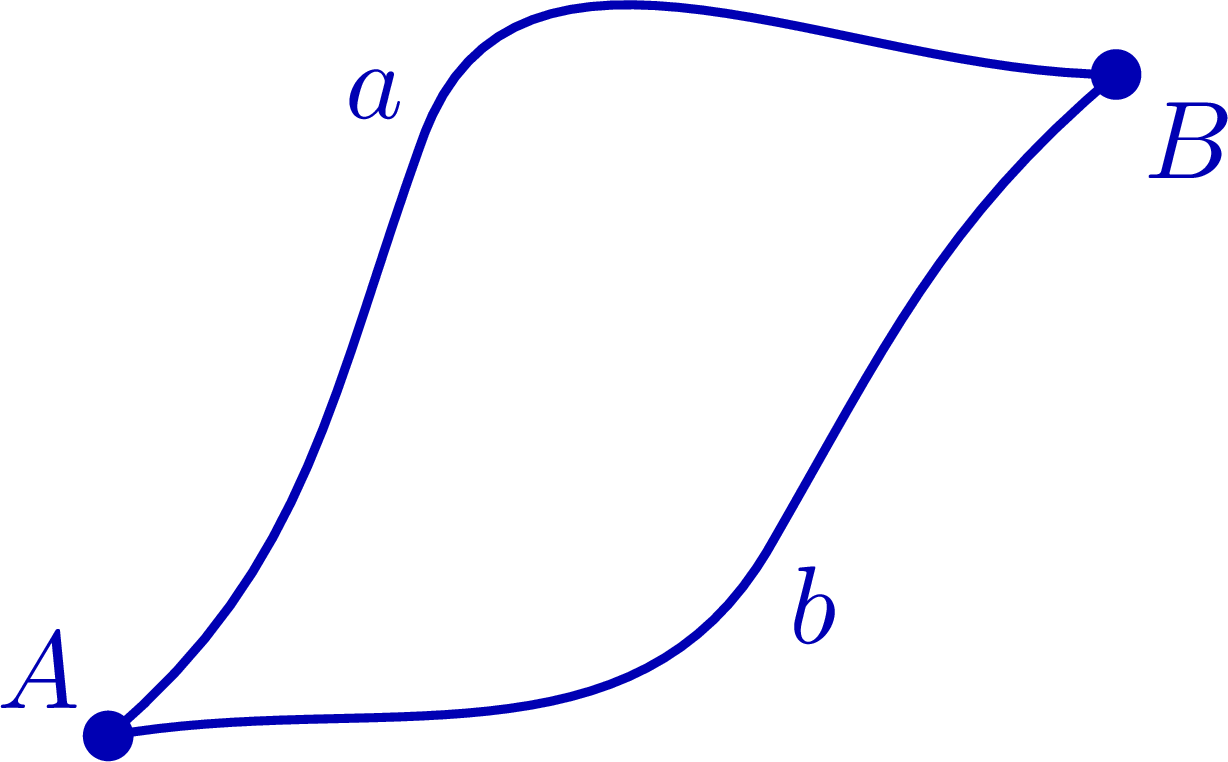
\includegraphics[width = 0.45 \textwidth]{image/lavoroNonDipDallaTraiett.png}
    \caption{Lavoro constante indipendentemente dal percorso scelto}
    \label{fig:lavoroCostante}
\end{figure}

\section{Energia Potenziale}
L'energia potenziale, $E_p$, è un tipo di energia che può essere associata solamente a corpi soggetti all'azione di forze conservative.
Essa è legata alla forza peso e all'altezza di caduta del corpo. Ha un limite: vale in prossimità della superficie terrestre.\\
Per definizione la variazione di energia potenziale è uguale al lavoro cambiato di segno: $\Delta E_p = -L$.\\
\paragraph{}
Per calcolare l'energia potenziale in un sistema si utilizza la seguente formula:
\begin{equation}
    E_p = mgh\quad[J = Nm]
    \label{energiaPotenziale}
\end{equation}

e le relative formule inverse:

\begin{equation}
    m = \frac{E_p}{gh}\quad[Kg] \qquad h= \frac{M_p}{mg}\quad\biggl[\frac{m}{s}\biggl]
\end{equation}

\paragraph{}
La formula \ref{energiaPotenziale} deriva dalla seguente dimostrazione.
\paragraph{}
Partiamo dalla formula della forza di gravità o forza peso:

\begin{equation*}
    \vec{F}=m\vec{g}
\end{equation*}
consideriamo $\vec{g}$ costante per quote vicine alla superficie terrestre.
Siccome la forza peso si esercita sempre verso il centro della terra, riscriviamo la forza considerando un sistema di riferimento con quote crescenti verso l'alto:
\begin{equation*}
    \vec{F}=-m\vec{g}
\end{equation*}

Utilizzando la definizione di energia potenziale, $\Delta E_p = -L$ otteniamo:

\begin{equation*}
     -L = \vec{F}\cdot\vec{dr}\footnote{$\vec{dr}$ rappresenta lo spostamento infinitesimo}
\end{equation*}

Dunque utilizzando gli integrai avremo che:

\begin{equation*}
     -\int_{h}^{0} dE_p = \int_{h}^{0} \vec{F} \cdot \vec{dr}
\end{equation*}
\begin{equation*}
    -[E_p]_h^0 = \int_{h}^{0} -mg dr
\end{equation*}
\begin{equation*}
     -E_p(0) + E_p(h) = mgh
\end{equation*}

\begin{equation}
    E_p(h) = E_p(0) + mgh
\end{equation}

\section{Energia Potenziale elastica}
L'energia potenziale elastica, $E_p$, è quell'energia che appartiene ad un corpo elastico come ad esempio la molla.
\e legata alla costante elastica $K$ e alla sua elongazione \footnote{Distanza lineare dalla posizione del copro in equilibrio}, l'energia potenziale elastica è sempre diretta in modulo opposto rispetto all'elongazione:

\begin{itemize}
    \item elongazione nulla, punto di equilibrio , $\Delta x = 0 \rightarrow$ forza nulla \hfill Figura \ref{fig:mollaAllung}
    \item elongazione positiva, allungamento, $\Delta x > 0 \rightarrow$ forza negativa \hfill Figura \ref{fig:mollaAllung}
    \item elongazione positiva, allungamento, $\Delta x < 0 \rightarrow$ forza positiva \hfill Figura \ref{fig:mollaAccoorc}
\end{itemize}

\paragraph{}
Per calcolare l'energia potenziale elastica in un sistema si utilizza la seguente formula:
\begin{equation}
    E_{pm} = \frac{1}{2}K(\Delta x)^2 \quad[J = Nm]
    \label{energiaPotenzialeElastica}
\end{equation}

e le relative formule inverse:

\begin{equation}
   K = \frac{2E_{pm}}{(\Delta x)^2}\quad\biggl[\frac{N}{m}\biggl] \qquad \Delta x = \sqrt{\frac{2E_{pm}}{K}}\quad[m]
\end{equation}

\paragraph{}
La formula \ref{energiaPotenzialeElastica} deriva dalla seguente dimostrazione:

Riprendendo la formula della forza elastica \ref{ForzaElastica} , $\vec{F_e} = -Kx $, e la definizione di energia potenziale $\Delta E_p = -L$ otteniamo:
\begin{equation*}
    \int_{x_0}^{0}-Kx\,dx = \int_{E_p(x_0)}^{E_p(0)} -dEp
\end{equation*}
\begin{equation*}
    -K\biggl[\frac{x^2}{2}\biggl]_{x_0}^{0} = -E_p(0) + E_p(x_0)
\end{equation*}
\begin{equation*}
    -K\biggl[\frac{x^2}{2}\biggl]_{x_0}^{0} = -E_p(0) + E_p(x_0)
\end{equation*}

L'energia potenziale elastica in $-E_p(0) = 0$, essendo la molla nel suo punto di equilibrio e dunque:
\begin{equation}
    K\frac{x_0^2}{2} = E_p(x_0)
\end{equation}


\begin{comment}
\begin{figure}
    \centering
    \begin{minipage}[c]{0.30\textwidth}
    \centering

        \begin{tikzpicture}
        
          \def\H{1.1}  % wall height
          \def\T{0.3}  % wall thickness
          \def\W{3.7}  % ground length
          \def\D{0.25} % ground depth
          \def\h{0.7}  % mass height
          \def\w{0.8}  % mass width
          \def\x{2.0}  % mass x position
          \def\y{1.22*\H} % x axis y position
          
          % AXIS
          \draw[mydashed] (\x,0.9*\h) --++ (0,\y-0.9*\h);
          \draw[axis] (\x-0.4*\W,\y) -- (\x+0.4*\W,\y) node[right] {$x$};
          \tick{\x,\y}{-90} node[scale=0.8,above=-1] {$0$};
          \draw[ell] (0,1.3*\h) --++ (\x,0) node[midway,fill=white,inner sep=0] {$\ell_0$};
          
          % SPRING & MASS
          \draw[spring] (0,\h/2) --++ (\x,0);
          \draw[ground] (0,0) |-++ (-\T,\H) |-++ (\T+\W,-\H-\D) -- (\W,0) -- cycle;
          \draw (0,\H) -- (0,0) -- (\W,0);
          \draw[mass] (\x,0) rectangle++ (\w,\h) node[midway] {$m$};
          
        \end{tikzpicture}
        
    \caption{Molla nel punto di equilibrio}
    \label{img:mollaEquilibrio}
    \end{minipage}
    \hspace{0.3mm}
    \begin{minipage}[c]{0.30\textwidth}
    \centering
        % HORIZONTAL spring - axis, extended
        \begin{tikzpicture}
          \def\H{1.1}  % wall height
          \def\T{0.3}  % wall thickness
          \def\W{3.9}  % ground length
          \def\D{0.25} % ground depth
          \def\h{0.7}  % mass height
          \def\w{0.8}  % mass width
          \def\x{2.0}  % mass x position
          \def\dx{0.8} % extension
          \def\y{1.22*\H} % x axis y position
          \def\F{0.8}  % force
          
          % AXIS
          \draw[mydashed] (\x,0) --++ (0,\y) (\x+\dx,0) --++ (0,1.1*\y);
          \draw[axis] (\x-0.4*\W,\y) -- (\x+0.4*\W,\y) node[right] {$x$};
          \tick{\x,\y}{-90} node[scale=0.8,above=-1] {$0$};
          \draw[ell] (0,1.3*\h) --++ (\x,0) node[midway,fill=white,inner sep=0] {$\ell_0$};
          \draw[dx] (\x,1.6*\h) --++ (\dx,0) node[pos=0.45,fill=white,inner sep=0] {$\Delta x$};
          
          % SPRING & MASS
          \draw[spring,segment length=7.5] (0,\h/2) --++ (\x+\dx,0);
          \draw[ground] (0,0) |-++ (-\T,\H) |-++ (\T+\W,-\H-\D) -- (\W,0) -- cycle;
          \draw (0,\H) -- (0,0) -- (\W,0);
          \draw[mass] (\x+\dx,0) rectangle++ (\w,\h) node[midway] {$m$};
          \draw[force] (\x+\dx+0.2*\w,0.9*\h) --++ (-\F,0) node[midway,right=1,above=-1] {$\vec{F}$};
          
        \end{tikzpicture}
    \caption{Molla allungata}
    \label{img:mollaAllungata}
    \end{minipage}
    \hspace{0.3mm}
    
    \begin{minipage}[c]{0.30\textwidth}
    \centering

% HORIZONTAL spring - axis, compressed
        \begin{tikzpicture}
          \def\H{1.1} % wall height
          \def\T{0.3} % wall thickness
          \def\W{3.9} % ground length
          \def\D{0.2} % ground depth
          \def\h{0.7} % mass height
          \def\w{0.8} % mass width
          \def\x{2.0} % mass x position
          \def\dx{0.9} % extension
          \def\y{1.22*\H} % x axis y position
          \def\F{0.8} % force
          
          % AXIS
          \draw[mydashed] (\x,0) --++ (0,\y) (\x-\dx,0) --++ (0,1.1*\y);
          \draw[axis] (\x-0.4*\W,\y) -- (\x+0.4*\W,\y) node[right] {$x$};
          \tick{\x,\y}{-90} node[scale=0.8,above=-1] {$0$};
          \draw[ell] (0,1.3*\h) --++ (\x,0) node[pos=0.4,fill=white,inner sep=0] {$\ell_0$};
          \draw[dx] (\x,1.6*\h) --++ (-\dx,0)
            node[pos=0.45,fill=white,inner sep=0,scale=0.9] {$\Delta x$};
          
          % SPRING & MASS
          \draw[spring,segment length=2.9] (0,\h/2) --++ (\x-\dx,0);
          \draw[ground] (0,0) |-++ (-\T,\H) |-++ (\T+\W,-\H-\D) -- (\W,0) -- cycle;
          \draw (0,\H) -- (0,0) -- (\W,0);
          \draw[mass] (\x-\dx,0) rectangle++ (\w,\h) node[midway] {$m$};
          \draw[force] (\x-\dx+0.8*\w,0.8*\h) --++ (\F,0) node[below=0,right=-1] {$\vec{F}$};
          
        \end{tikzpicture}
    
    \caption{Molla nel punto di equilibrio}
    \label{img:mollaEquilibrio}
    \end{minipage}
\end{figure}
\end{comment}

\begin{figure}[H]
    \centering
        % HORIZONTAL spring - axis, rest position
    \begin{tikzpicture}[scale = 1.3]
      \def\H{1.1}  % wall height
      \def\T{0.3}  % wall thickness
      \def\W{3.7}  % ground length
      \def\D{0.25} % ground depth
      \def\h{0.7}  % mass height
      \def\w{0.8}  % mass width
      \def\x{2.0}  % mass x position
      \def\y{1.22*\H} % x axis y position
      
      % AXIS
      \draw[mydashed] (\x,0.9*\h) --++ (0,\y-0.9*\h);
      \draw[axis] (\x-0.4*\W,\y) -- (\x+0.4*\W,\y) node[right] {$x$};
      \tick{\x,\y}{-90} node[scale=0.8,above=-1] {$0$};
      \draw[ell] (0,1.3*\h) --++ (\x,0) node[midway,fill=white,inner sep=0] {$\ell_0$};
      
      % SPRING & MASS
      \draw[spring] (0,\h/2) --++ (\x,0);
      \draw[ground] (0,0) |-++ (-\T,\H) |-++ (\T+\W,-\H-\D) -- (\W,0) -- cycle;
      \draw (0,\H) -- (0,0) -- (\W,0);
      \draw[mass] (\x,0) rectangle++ (\w,\h) node[midway] {$m$};
      
    \end{tikzpicture}
    \caption{Molla nel punto di equilibrio}
        \label{fig:mollaEquilibrio}
    
    % HORIZONTAL spring - axis, extended
    \begin{tikzpicture}[scale = 1.3]
      \def\H{1.1}  % wall height
      \def\T{0.3}  % wall thickness
      \def\W{3.9}  % ground length
      \def\D{0.25} % ground depth
      \def\h{0.7}  % mass height
      \def\w{0.8}  % mass width
      \def\x{2.0}  % mass x position
      \def\dx{0.8} % extension
      \def\y{1.22*\H} % x axis y position
      \def\F{0.8}  % force
      
      % AXIS
      \draw[mydashed] (\x,0) --++ (0,\y) (\x+\dx,0) --++ (0,1.1*\y);
      \draw[axis] (\x-0.4*\W,\y) -- (\x+0.4*\W,\y) node[right] {$x$};
      \tick{\x,\y}{-90} node[scale=0.8,above=-1] {$0$};
      \draw[ell] (0,1.3*\h) --++ (\x,0) node[midway,fill=white,inner sep=0] {$\ell_0$};
      \draw[dx] (\x,1.6*\h) --++ (\dx,0) node[pos=0.45,fill=white,inner sep=0] {$\Delta x$};
      
      % SPRING & MASS
      \draw[spring,segment length=7.5] (0,\h/2) --++ (\x+\dx,0);
      \draw[ground] (0,0) |-++ (-\T,\H) |-++ (\T+\W,-\H-\D) -- (\W,0) -- cycle;
      \draw (0,\H) -- (0,0) -- (\W,0);
      \draw[mass] (\x+\dx,0) rectangle++ (\w,\h) node[midway] {$m$};
      \draw[force] (\x+\dx+0.2*\w,0.9*\h) --++ (-\F,0) node[midway,right=1,above=-1] {$\vb{-F}$};
      
    \end{tikzpicture}
    \caption{Molla allungata}
        \label{fig:mollaAllung}
    
    % HORIZONTAL spring - axis, compressed
    \begin{tikzpicture}[scale = 1.3]
      \def\H{1.1} % wall height
      \def\T{0.3} % wall thickness
      \def\W{3.9} % ground length
      \def\D{0.2} % ground depth
      \def\h{0.7} % mass height
      \def\w{0.8} % mass width
      \def\x{2.0} % mass x position
      \def\dx{0.9} % extension
      \def\y{1.22*\H} % x axis y position
      \def\F{0.8} % force
      
      % AXIS
      \draw[mydashed] (\x,0) --++ (0,\y) (\x-\dx,0) --++ (0,1.1*\y);
      \draw[axis] (\x-0.4*\W,\y) -- (\x+0.4*\W,\y) node[right] {$x$};
      \tick{\x,\y}{-90} node[scale=0.8,above=-1] {$0$};
      \draw[ell] (0,1.3*\h) --++ (\x,0) node[pos=0.4,fill=white,inner sep=0] {$\ell_0$};
      \draw[dx] (\x,1.6*\h) --++ (-\dx,0)
        node[pos=0.45,fill=white,inner sep=0,scale=0.9] {$\Delta x$};
      
      % SPRING & MASS
      \draw[spring,segment length=2.9] (0,\h/2) --++ (\x-\dx,0);
      \draw[ground] (0,0) |-++ (-\T,\H) |-++ (\T+\W,-\H-\D) -- (\W,0) -- cycle;
      \draw (0,\H) -- (0,0) -- (\W,0);
      \draw[mass] (\x-\dx,0) rectangle++ (\w,\h) node[midway] {$m$};
      \draw[force] (\x-\dx+0.8*\w,0.8*\h) --++ (\F,0) node[below=0,right=-1] {$\vb{+F}$};
      \end{tikzpicture}
    \caption{Molla accorciata}
    \label{fig:mollaAccoorc}
\end{figure}

\section{Energia meccanica}
Energia meccanica, indicata con il simbolo $E$, è la somma dell’energia cinetica e dell’energia potenziale. Solo in presenza di forze conservative vale il principio di conservazione dell’energia secondo cui l’energia meccanica  ($E$ o $E_{tot}$) si conserva.

\begin{equation}
    E = E_p + E_c
\end{equation}

Infatti:
Il lavoro dell'energia cinetica e potenziale è così definito:

\begin{equation*}
    L = E_{cf} - E_{ci} \qquad -L = E_{pf} - E_{pi}
\end{equation*}

da cui: 

\begin{equation*}
    E_{cf} - E_{ci} = -E_{pf} + E_{pi}
\end{equation*}
\begin{equation*}
    E_{cf} + E_{pf} = E_{pi} + E_{ci}
\end{equation*}
\begin{equation}
    E_f = E_i
\end{equation}

Quindi abbiamo trovato che la somma dell'energia cinetica e potenziale, allo stato iniziale, è uguale alla somma dell'energia cinetica e potenziale allo stato finale.


\section{Potenza}
La potenza in Fisica, indicata con il simbolo $P$, è una grandezza legata al concetto di lavoro che fornisce una misura di quanto lavoro è stato svolto in un'unità di tempo.
Nel SI l'unità di misura della potenza è il Watt, $W = \frac{J}{s}$.

Il termine potenza o $W$ che comunemente viene utilizzato nel linguaggio comune, come ad esempio per compiere uno sforzo fisico o meccanico, non è molto diverso dal concetto fisico.

Per calcolare la potenza si utilizza la seguente formula:

\begin{equation}
    P = \frac{L}{\Delta t} = \frac{\vec{F} \cdot \vec{dr}}{dt} = \vec{F}\cdot \vec{v}\qquad \biggl[ W = \frac{J}{s}\biggl]
\end{equation}


\section{Pendolo semplice}

\def\L{2.8}  % string length
\def\ang{28} % angle string
\def\R{0.25} % ball radius
\def\F{1.0}  % force magnitude
\begin{figure}[H]
    \centering
    \begin{tikzpicture}
      \message{^^JPendulum}
      \coordinate (M) at (\ang-90:\L);
      \coordinate (M') at (0,-\L);
      \coordinate (O) at (0,0);
      \coordinate (B) at (0,-\L-2.2*\R);
      \coordinate (FT) at ($(M)+(90+\ang:{\F*cos(\ang)+\R})$);
      \coordinate (FG) at ($(M)+(-90:{\F+\R})$);
      \coordinate (FGx) at ($(M)+(-90+\ang:{0.55*\F+\R})$);
      \coordinate (MA) at ($(M)+(180+\ang:{\F*sin(\ang)+\R})$);
      %\draw[faded mass] (M') circle(\R);
      \draw[<->] (M)++(\ang-32:0.2*\L) node[below right=-1,scale=0.9] {$x$}
        --++ (\ang:0.17*\L) --++ (90+\ang:0.17*\L) node[above right=-1,scale=0.9] {$y$};
      \draw[dashed] (O) -- (B);
      %\draw[dashed,myred!60!black] (MA) -- (FG);
      \draw[dashed,myred!60!black] (M) -- (FGx);
      \draw[dashed] (-90+\ang+10:\L) arc(-90+\ang+10:-110:\L) (B);
      \rope{(O) -- (M)} \path (O) -- (M) node[midway,above right=-1] {$L$};
      \fill[black] (O) circle(0.04);
      \draw[force] (M) -- (FT) node[midway,left=0] {$\vb{T}$};
      \draw[force] (M) -- (FG) node[right=0] {$m\vb{g}$};
      \draw[force,acol] (M) -- (MA) node[right=2,below=0] {$m\vb{a}$}; %{\contour{white}{$m\vb{a}$}};
      \draw[mass] (M) circle(\R) node {$m$};
      \draw pic[myarr,"$\theta$",xcol,draw=xcol,angle radius=22,angle eccentricity=1.30] {angle=B--O--M}; %_\text{max}
      \draw pic[myarr,"$\theta$",xcol,draw=xcol,angle radius=14,angle eccentricity=1.45] {angle=FG--M--FGx};
    \end{tikzpicture}
    \caption{Pendolo semplice}
    \label{fig:pendoloSemplice}
\end{figure}

Il pendolo semplice è formato da una massa $m$ attaccato a un filo di lunghezza $L$. Il pendolo è in equilibrio stabile quando la massa si trova esattamente sotto al punto di sospensione e oscilla attorno a tale punto. 
Il pendolo gode di un moto armonico, ovvero impiega sempre lo stesso tempo a compiere un oscillazione completa.

\begin{figure}[H]
    \centering
    \begin{tikzpicture}[scale = 1.3]
      \message{^^JPendulum forces}
      \def\F{1.4}  % force magnitude
      \coordinate (O) at (0,0);
      \coordinate (FT) at (90+\ang:{\F*cos(\ang)});
      \coordinate (FG) at (-90:\F);
      \coordinate (FGx) at (-90+\ang:{\F*cos(\ang)});
      \coordinate (FGy) at (180+\ang:{\F*sin(\ang)});
      \draw[dashed,myred!60!black] (FGy) -- (FG); %-- (FGx);
      \draw[force] (O) -- (FT) node[midway,above right=-2] {$\vb{T}$};
      \draw[Fproj] (O) -- (FGy) node[pos=0.4,above left=-3,scale=0.86] {$mg\sin\theta$};
      \draw[Fproj] (O) -- (FGx) node[pos=0.5,above right=-3,scale=0.86] {$mg\cos\theta$};
      \draw[force] (O) -- (FG) node[right=0] {$m\vb{g}$};
      \draw pic[myarr,"$\theta$",xcol,draw=xcol,angle radius=14,angle eccentricity=1.45] {angle=FG--O--FGx};
    \end{tikzpicture}
    \caption{Forze applicate alla massa $m$ del pendolo in Figura \ref{fig:pendoloSemplice}}
    \label{fig:forzePendolo}
\end{figure}

\paragraph{}
Consideriamo ora le forze che agiscono sulla massa $m$, rappresentate nella figura \ref{fig:forzePendolo}.
Vediamo che sono rappresentate la forza peso e la tensione della filo. La tensione agisce in direzione radiale \footnote{Nella stessa direzione del raggio} e la sua intensità è uguale alla componente radiale del peso.

\begin{equation}
    T = mg\cos\theta
\end{equation}

La forza tangenziale che agisce sulla massa $m$ è sempre diretta verso il punto di equilibrio del pendolo: sotto al punto di sospensione.

\begin{equation}
    F = mg\sin\theta
\end{equation}

Inoltre per il \textit{Teorema dei piccoli angoli} fino a angoli di $30\gradi$ possiamo approssimare:
\begin{equation*}
    \sin\theta \approx \theta \qquad \text{$\theta$ è in radianti}
\end{equation*}

grazie agli sviluppi di Taylor:

\begin{equation*}
    \sin\theta = \theta - \frac{\theta^3}{6} + ...
\end{equation*}

Fermandoci al primo ordine avremo che:

\begin{equation*}
    \sin 30\gradi = 0.5 \quad\text{e dallo sviluppo ricaviamo}\quad 30\gradi  =  0,52 \,\text{Rad}
\end{equation*}

con un errore massimo di due centesimi, dato da $\frac{(\sin\theta)^3}{6} = 0.02$

\paragraph{}
Formule utili per la risoluzione dei problemi:
\paragraph{}
Velocità angolare:
\begin{equation}
    \omega = \sqrt{\frac{g}{L}}\quad \biggl[\frac{Rad}{s}\biggl]\qquad \omega = \sqrt{\frac{g}{L}}\frac{1}{2\pi}\quad \biggl[\frac{Giri}{s}\biggl]
\end{equation}

Periodo:
\begin{equation}
    P = 2\pi \sqrt{\frac{L}{g}} = \frac{2\pi}{\omega}
\end{equation}

Tensione \footnote{La tensione è massima quando $\theta = 0$}
\begin{equation}
    T = mg\cos\theta + mL\omega^2 = mg\cos\theta + m\frac{v^2}{L}
\end{equation}
viene usata l'accelerazione centripeta di pagina \pageref{AccelerazioneCentripeta}.
\paragraph{}
Conservazione dell'energia:
\begin{equation}
    mg(L-L\cos\theta_{max}) = \frac{1}{2}mv_{max}^2
\end{equation}
si veda la Figura \ref{fig:conservazioneEnergiaPendolo}
\paragraph{}
Velocità massima:
\begin{equation}
    v_{max} = \sqrt{2gL(1-\cos\theta_{max})}
\end{equation}

\def\L{2.8} % length
    \def\ang{32} % length
    \def\R{0.25} % ball radius
\begin{figure}[tb]
    \centering
    \begin{tikzpicture}[scale=1.3]
      \coordinate (M) at (\ang-90:\L);
      \coordinate (M') at (0,-\L);
      \coordinate (O) at (0,0);
      \coordinate (B) at (0,-\L-1.4*\R);
      \draw[faded mass] (M') circle(\R);
      \draw[dashed] (O) -- (B);
      \draw[dashed] (M')++(-0.7*\R,0) --++ ({0.65*\L*sin(\ang)},0) coordinate (A);
      \draw[dashed] (M')++(-0.7*\R,{\L-\L*cos(\ang)}) --++ ({1.2*\L*sin(\ang)},0);
      \draw[<->] (A)++(-0.2*\R,0) --++ (0,{\L-\L*cos(\ang)}) node[midway,right=-1] {$h$};
      \rope{(O) -- (M)} \path (O) -- (M) node[midway,right=1] {$L$};
      \fill[black] (O) circle(0.04);
      %\draw[force] (M)++(140:0.7*\r) --++ (-\F,0) node[below=1,above left=-4] {$\vb{F}_\mathrm{c}$};
      \draw[mass] (M) circle(\R) node {$m$};
      \draw pic[->,"\,$\theta_\text{max}$",xcol,draw=xcol,angle radius=29,angle eccentricity=1.3] {angle=B--O--M};
    \end{tikzpicture}
    \caption{Conservazione energia del pendolo}
    \label{fig:conservazioneEnergiaPendolo}
\end{figure}

\newpage
\section{Conservazione della quantità di moto}

Fino ad ora ci siamo interessati solo di come un corpo si muove su un piano soggetto a delle forze che agivano su di esso.
In questo capitolo ci concentreremo su cosa succede quando ci sono più corpi che interagiscono gli uni con gli altri per la terza legge di Newton \ref{terzaLeggeNewton}. 

Per prima cosa diamo la definizione di sistema: 
in fisica un sistema è un qualsiasi insieme di oggetti o punti materiali presi singolarmente. Esempio: un atomo o un pezzo continuo di materia come un cubo di lato 10 cm.

Questi punti materiali sono soggetti a forze interne e forze esterne:
\begin{itemize}
    \item Forza Interna: forza intrinsecamente presente nel sistema ($3^a$ Legge di Newton)
    \item Forza Esterna: forza applicata al di fuori del sistema, sono le interazioni esterne
\end{itemize}

La quantità di moto di un corpo di massa $m$ che si muove a velocità $\vec{v}$ è il vettore:

\begin{equation}
    \vec{p} = m\vec{v} \qquad\biggl[Kg\frac{m}{s}\biggl]
\end{equation}


\begin{figure}[H]
    \centering
    % GRAVITATIONAL ATTRACTION
    \begin{tikzpicture}
      \def\d{4.1}  % distance r
      \def\r{0.3}  % small radius ball
      \def\R{0.38} % large radius ball
      \def\RR{0.35} % large radius ball
      \def\F{0.95} % force magnitude
      \def\u{0.4}  % unit vector magnitude
      \def\ang{5}  % angle lin
      \coordinate (M1) at (0,0);
      \coordinate (M2) at (\ang:\d);
      \coordinate (M3) at (2,-1.8);
      
      % SETUP
      \draw[mass] (M1) circle(\r) node[scale=0.9] {$m_1$};
      \draw[mass] (M2) circle(\R) node[scale=0.9] {$m_2$};
      \draw[mass] (M3) circle(\RR) node[scale=0.9] {$m_3$};
      
      % FORCES
      \draw[force] (M1)++(\ang-8:0.9*\r) --++ (\ang:\F)
        node[anchor=90,inner sep=4] {$\vbF_{12}$}; % = -G\dfrac{m_1m_2}{r^2}\vu{r}_{21}
      \draw[force] (M2)++(\ang-172:0.9*\R) --++ (\ang:-\F)
        node[anchor=130,inner sep=3] {$\vbF_{21}$}; % = -G\dfrac{m_1m_2}{r^2}\vu{r}_{12}
        
        %est
        \draw[force] (M1)++(\ang0:0.3) --++ (\ang+25:0.9)
        node[anchor=90,inner sep=6] {$\vbF_{EST}$}; % = -G\dfrac{m_1m_2}{r^2}\vu{r}_{21}
        
        \draw[force] (M1)++(\ang-800:0.9*\r) --++ (\ang-50:0.9)
        node[anchor=20,inner sep=2] {$\vbF_{13}$}; % = -G\dfrac{m_1m_2}{r^2}\vu{r}_{21}
        
        %est
        \draw[force] (M2)++(\ang-80:0.4) --++ (\ang-100:0.9)
        node[anchor=90,inner sep=4] {$\vbF_{EST}$}; % = -G\dfrac{m_1m_2}{r^2}\vu{r}_{21}
      \draw[force] (M2)++(\ang99:0.9*\R) --++ (\ang-140:0.9)
        node[anchor=190,inner sep=10] {$\vbF_{23}$}; % = -G\dfrac{m_1m_2}{r^2}\vu{r}_{12}
        
        \draw[force] (M3)++(\ang+40:0.35) --++ (\ang+40:0.9)
        node[anchor=-250,inner sep=6] {$\vbF_{32}$}; % = -G\dfrac{m_1m_2}{r^2}\vu{r}_{21}
        
        %est
        \draw[force] (M3)++(\ang-150:0.35) --++ (\ang-190:0.9)
        node[anchor=90,inner sep=4] {$\vbF_{EST}$}; % = -G\dfrac{m_1m_2}{r^2}\vu{r}_{21}
      \draw[force] (M3)++(\ang-5:-0.35) --++ (\ang+130:0.9)
        node[anchor=190,inner sep=5] {$\vbF_{31}$}; % = -G\dfrac{m_1m_2}{r^2}\vu{r}_{12}
      
    \end{tikzpicture}
    \caption{Sistema di oggetti}
    \label{fig:sistemaOggetti}
\end{figure}


La forza totale che agisce sui corpi del sistema è la seguente:
\begin{equation*}
    m_1\veca_1 = \vec{F_{12}} + \vec{F_{13}} + \vec{F_{1est}}
\end{equation*}
\begin{equation*}
    m_2\veca_2 = \vec{F_{21}} + \vec{F_{23}} + \vec{F_{2est}}
\end{equation*}
\begin{equation*}
    m_3\veca_3 = \vec{F_{31}} + \vec{F_{32}} + \vec{F_{3est}}
\end{equation*}

tutte le coppie opposte si elidono e rimane solo:

\begin{equation*}
     m_1\veca_1 + m_2\veca_2+  m_3\veca_3 = \vec{F_{1est}} +\vec{F_{2est}} + \vec{F_{3est}}
\end{equation*}
\begin{equation}
    \sum_{i = 1} ^ 3 m_i\veca_i = \sum_{i = 1} ^ 3 m_i\vec{F_{iest}}
\end{equation}

Da questo capiamo che la somma delle forze interne è nulla e la quantità di moto totale dipende solo dalla somma delle forze esterne al sistema.
Quando siamo in presenza di un sistema isolato, cioè non è soggetto a forze esterne, allora anche la risultante della somma delle forze estere è nulla da cui abbiamo che:
\begin{equation}
    0 = \sum \vec{F_{int}} = \sum \vec{F_{est}} = 0
\end{equation}
Questo significa che la quantità di moto totale in un sistema isolato rimane costante:
\begin{equation}
    \vec{p}_{i-tot} = \vec{p}_{f-tot}
\end{equation}

\subsection{Il lavoro delle forze interne}
Le forze interne non alterano la quantità di moto totale di un sistema, ma in genere producono effetti sui singoli corpi che formano il sistema, infatti ogni variazione di energia cinetica corrisponde ad una variazione uguale di altre forze di energia all'intero del sistema stesso.
 Si pensi ad esempio ad un bagnino in piedi su una barca che lancia un salvagente, la barca acquista velocità ma a sua volta il salvagente compie un lavoro sul sistema barca + bagnino, che acquista energia cinetica. L’energia cinetica del salvagente è uguale all'energia chimica prodotta dai muscoli durante il lancio.
 
 \subsection{Centro di massa}
 La maggior parte degli oggetti comuni non sono punti, ma prendono le più svariate forme e dimensioni.
 In fisica questi corpi possono essere considerati come un sistema di corpi puntiformi e per analizzare il moto di un sistema di massa è utile considerare un particolare punto detto \textit{centro di massa} o \textit{baricentro}.
 
 La conservazione della quantità di moto ha un profondo effetto sui moti del baricentro, infatti questo punto si muove come il sistema puntiforme iniziale soggetto alle medesime forze esterne.
 
 Il baricentro di un sistema isolato si muove di moto rettilineo uniforme.
 
 \section{Urti}
 Un urto è un’interazione fra due corpi che vengono a contatto per un breve periodo di tempo.
 La conservazione della quantità di moto è uno strumento fondamentale per analizzare le dinamiche degli urti, permette di relazionare le velocità prima e dopo gli urti: in altri termini la quantità di moto del sistema immediatamente prima dell'impatto è uguale alla quantità di moto del sistema dopo l’impatto.
 
 \subsection{Urto anelastico}
 \e un urto dove non si conserva l’energia cinetica totale, in particolare se rimangono attaccati si parla di urto completamente anelastico e quindi i due corpi avranno la medesima velocità finale.
 
 La quantità di moto si conserva, energia cinetica non si conserva.
 
 \paragraph{}
 Formule per la risoluzione:
 \paragraph{}
 Urto anelastico:
\begin{equation}
    m_1\vec{v_1i} + m_2\vec{v_2i} = m_1\vec{v_1f} + m_2\vec{v_2f}
\end{equation}
nel caso l'urto sia anelastico si devono sapere tutte le quattro variabili dell'equazione precedente

\begin{figure}[H]
    \centering
    \def\w{0.8} % mass width
    \def\h{0.5} % mass height
    \def\v{0.7} % mass velocity
    \def\L{4.6} % length
    \begin{tikzpicture}
      \def\d{2.2} % distance
      \coordinate (M1) at (-\d/2+\w/2,0);
      \coordinate (M2) at (\d/2-\w/2,0);
      \draw[ground] (-\L/2,0) rectangle++ (\L,-0.2);
      \draw[thick] (-\L/2,0) --++ (\L,0);
      \draw[velocity] (M1)++(-\w/2,\h/2) --++ (-0.8*\v,0) node[left=-2] {$\vb{v}'_1$};
      \draw[velocity] (M2)++(\w/2,\h/2) --++ (1.2*\v,0) node[right=-2] {$\vb{v}'_2$};
      \draw[mass] (M1)++(-\w/2,0) rectangle++ (\w,\h) node[midway] {$m_1$};
      \draw[mass] (M2)++(-\w/2,0) rectangle++ (\w,\h) node[midway] {$m_2$};
      \pic[scale=1] at (0,0.5*\h) {collision={0.8}};
    \end{tikzpicture}
    \caption{Urto anelastico}
    \label{fig:UrtoAnelastico}
\end{figure}

\paragraph{}
 Urto completamente anelastico:
\begin{equation}
    m_1\vec{v_1i} + m_2\vec{v_2i} = (m_1+ m_2)\vec{v_f}
\end{equation}
in alcuni casi si deve mettere a sistema questa equazione con il moto rettilineo uniformemente accelerato \ref{leggeOrunifacc}

 \begin{figure}[H]
     \centering
     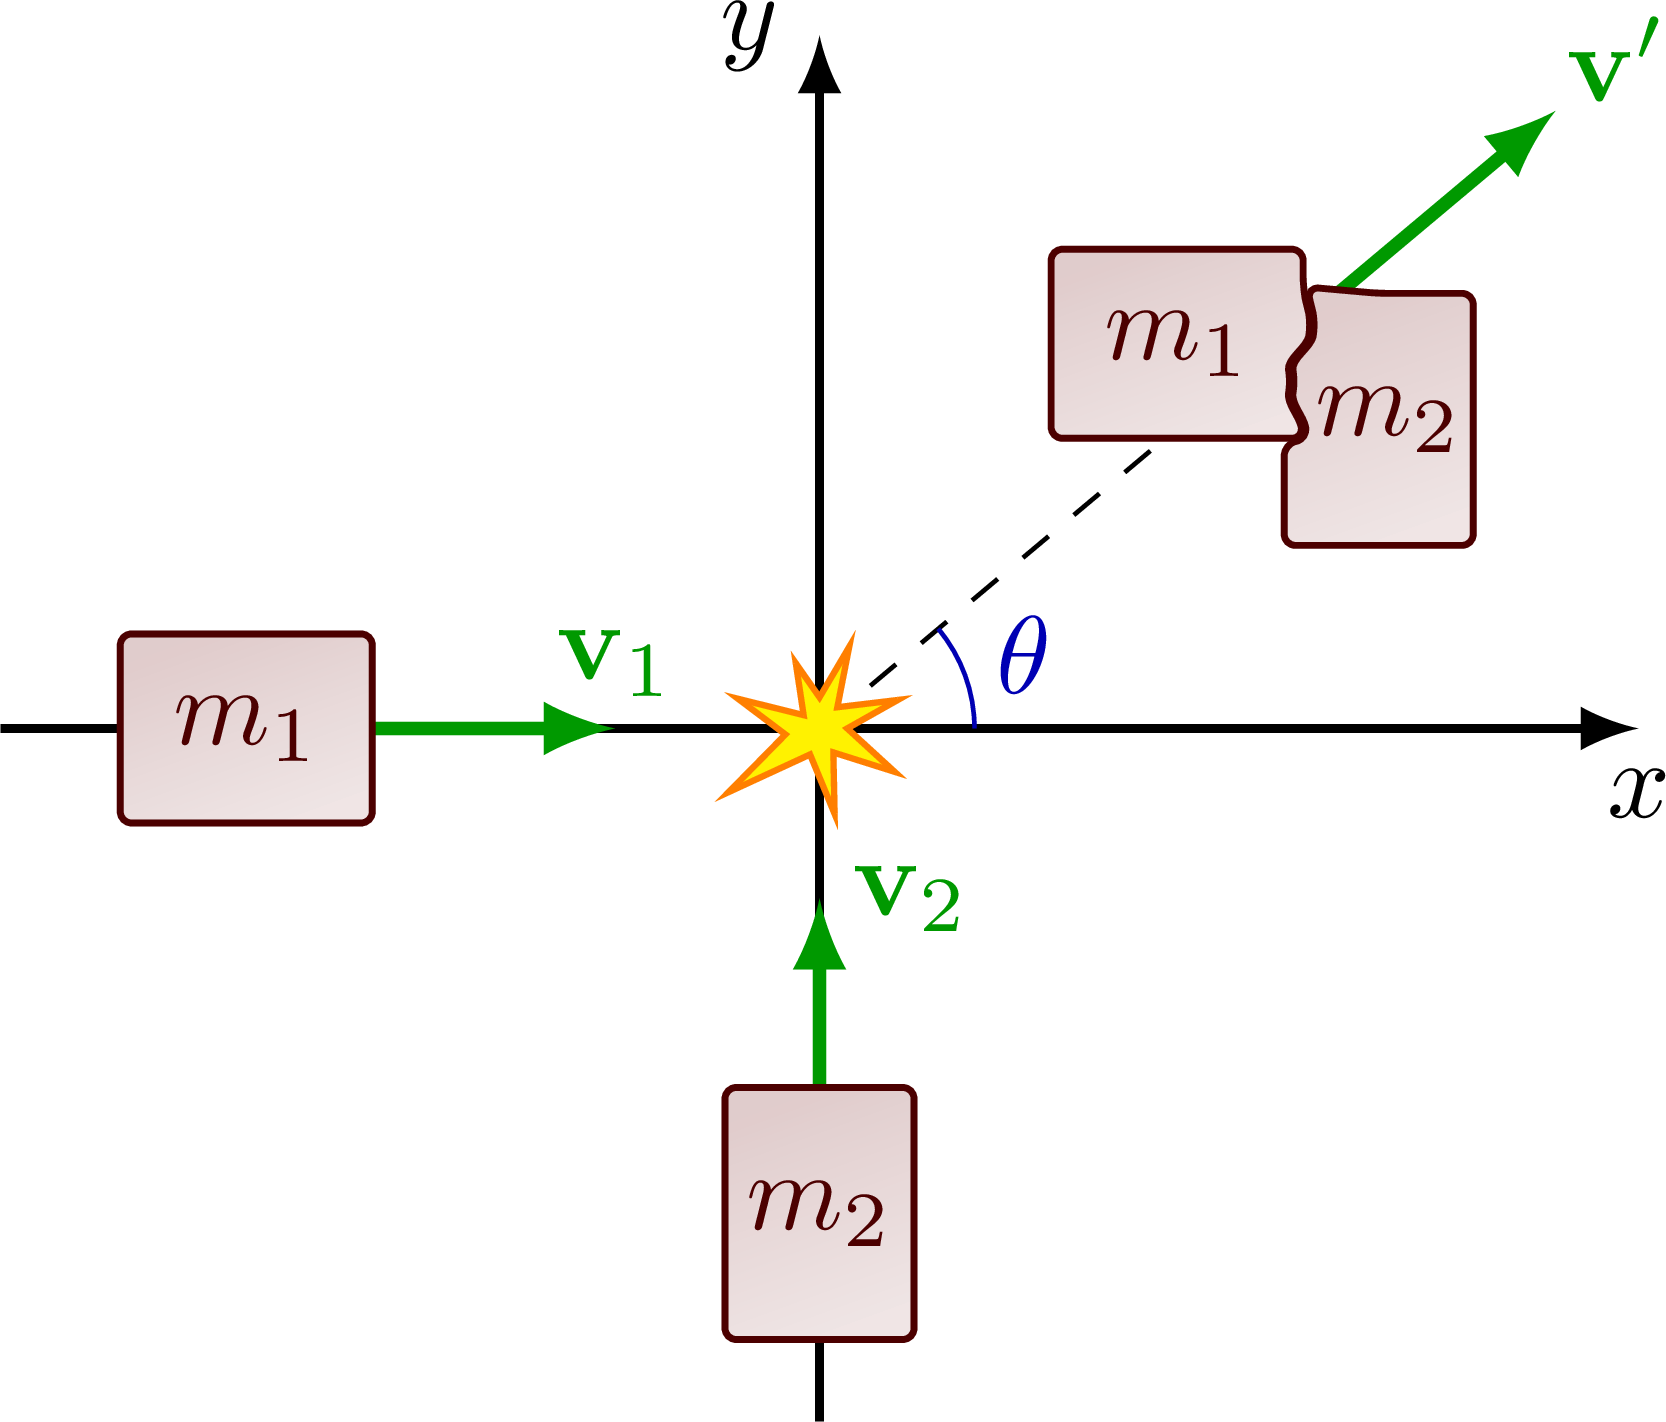
\includegraphics[width = 0.45\textwidth]{image/urtoAnelastico.png}
     \caption{Urto completamente anelastico}
     \label{fig:urtocompletamenteAnelastico}
 \end{figure}
 
\subsection{Urto elastico}
L’urto elastico è un urto dove si conserva sia la quantità di moto che l’energia cinetica. Si pensi al biliardo.

\paragraph{}
 Urto elastico:
$$
\begin{cases}

    m_1\vec{v_1i} + m_2\vec{v_2i} = m_1\vec{v_1f} + m_2\vec{v_2f}\\[10pt]
    \frac{1}{2}m_1\vec{v_1i}^2 + \frac{1}{2}m_2\vec{v_2i}^2  =\frac{1}{2}m_1\vec{v_1f}^2 + \frac{1}{2}m_2\vec{v_2f}^2
     
\end{cases}
$$

Mettiamo a sistema la quantità di moto con l'energia potenziale.

\paragraph{}
Troviamo le velocità finali dei due corpi:
$$
\begin{cases}

    v_{1f} = \frac{m1 -m2}{m1+m2}v_{1i} + \frac{2m_2}{m1+m2}v_{2i}\\[10pt]
    v_{2f} = \frac{m2 -m1}{m1+m2}v_{2i} + \frac{2m_1}{m1+m2}v_{1i}\\
     
\end{cases}
$$

Alcuni esempi...

\begin{figure}[H]
\centering
    \begin{minipage}[c]{0.45\textwidth}
    \centering
    % COLLISION 1D before
    \def\w{0.8} % mass width
    \def\h{0.5} % mass height
    \def\v{0.7} % mass velocity
    \def\L{4.6} % length
    \begin{tikzpicture}
      \def\d{3.8} % distance
      \coordinate (M1) at (-\d/2+\w/2,0);
      \coordinate (M2) at (\d/2-\w/2,0);
      \draw[ground] (-\L/2,0) rectangle++ (\L,-0.2);
      \draw[thick] (-\L/2,0) --++ (\L,0);
      \draw[velocity] (M1)++(\w/2,\h/2) --++ (1.1*\v,0) node[left=2,above=0] {$\vb{v}_1$};
      \draw[mass] (M1)++(-\w/2,0) rectangle++ (\w,\h) node[midway] {$m$};
      \draw[mass] (M2)++(-\w/2,0) rectangle++ (\w,\h) node[midway] {$m$};
    \end{tikzpicture}
    \caption{Urto elastico masse uguali, prima}
    \label{fig:urtoElasticoMasseUguali}
    \end{minipage}
    \hspace{0.1mm}
    \begin{minipage}[c]{0.45\textwidth}
    \centering
    % COLLISION 1D before
    \def\w{0.8} % mass width
    \def\h{0.5} % mass height
    \def\v{0.7} % mass velocity
    \def\L{4.6} % length
    \begin{tikzpicture}
      \def\d{3.8} % distance
      \coordinate (M1) at (-\d/2+\w/2,0);
      \coordinate (M2) at (\d/2-\w/2,0);
      \draw[ground] (-\L/2,0) rectangle++ (\L,-0.2);
      \draw[thick] (-\L/2,0) --++ (\L,0);
      \draw[mass] (M2)++(-\w/2,0) rectangle++ (\w,\h) node[midway] {$m$};
    \end{tikzpicture}
    \caption{Urto elastico masse uguali, dopo}
    \label{fig:urtoElasticoMasseUgualiDopo}
    \end{minipage}
    
\end{figure}

In Figura \ref{fig:urtoElasticoMasseUguali} viene rappresentato un urto elastico tra due blocchi di massa $m$.
Dopo l'urto, in accordo con le formule, troveremo che il blocco in movimento si sarà fermato ed avrà sostituito il posto del blocco fermo il quale ha iniziato a muoversi verso destra con velocità pari a $\vec{v_1}$.


\begin{figure}[H]
\centering
    \begin{minipage}[c]{0.45\textwidth}
    \centering
    % COLLISION 1D before
    \def\w{0.8} % mass width
    \def\h{0.5} % mass height
    \def\v{0.7} % mass velocity
    \def\L{4.6} % length
    \begin{tikzpicture}
      \def\d{3.8} % distance
      \coordinate (M1) at (-\d/2+\w/2,0);
      \coordinate (M2) at (\d/2-\w/2,0);
      \draw[ground] (-\L/2,0) rectangle++ (\L,-0.2);
      \draw[thick] (-\L/2,0) --++ (\L,0);
      \draw[velocity] (M1)++(\w/2,\h/2) --++ (1.1*\v,0) node[left=2,above=0] {$\vb{v}_1$};
      \draw[mass] (M1)++(-\w/2,0) rectangle++ (\w,\h) node[midway] {$M$};
      \draw[mass] (M2)++(-\w/2,0) rectangle++ (\w,\h) node[midway] {$m$};
    \end{tikzpicture}
    \caption{Urto elastico masse diverse, prima}
    \label{fig:urtoElasticoMasseDiversi}
    \end{minipage}
    \hspace{0.1mm}
    \begin{minipage}[c]{0.45\textwidth}
    \centering
    % COLLISION 1D before
    \def\w{0.8} % mass width
    \def\h{0.5} % mass height
    \def\v{0.7} % mass velocity
    \def\L{4.6} % length
    \begin{tikzpicture}
      \def\d{3.8} % distance
      \coordinate (M1) at (-\d/2+\w/2,0);
      \coordinate (M2) at (\d/2-\w/2,0);
      \draw[ground] (-\L/2,0) rectangle++ (\L,-0.2);
      \draw[thick] (-\L/2,0) --++ (\L,0);
    \end{tikzpicture}
    \caption{Urto elastico masse diverse, dopo}
    \label{fig:urtoElasticoMasseDiversiDopo}
    \end{minipage}
    
\end{figure}
In Figura \ref{fig:urtoElasticoMasseDiversi} viene rappresentato un urto elastico tra due blocchi di massa $M$ e massa $m$.
Dopo l'urto troveremo che il blocco in movimento, siccome molto più massivo dell'oggetto fermo, avrà travolto $m$ continuando ad una velocità pressoché inalterata a $\vec{v_1}$.

\begin{figure}[H]
\centering
    \begin{minipage}[c]{0.45\textwidth}
    \centering
    % COLLISION 1D before
    \def\w{0.8} % mass width
    \def\h{0.5} % mass height
    \def\v{0.7} % mass velocity
    \def\L{4.6} % length
    \begin{tikzpicture}
      \def\d{3.8} % distance
      \coordinate (M1) at (-\d/2+\w/2,0);
      \coordinate (M2) at (\d/2-\w/2,0);
      \draw[ground] (-\L/2,0) rectangle++ (\L,-0.2);
      \draw[thick] (-\L/2,0) --++ (\L,0);
      \draw[velocity] (M1)++(\w/2,\h/2) --++ (1.1*\v,0) node[left=2,above=0] {$\vb{v}_1$};
      \draw[mass] (M1)++(-\w/2,0) rectangle++ (\w,\h) node[midway] {$m$};
      \draw[mass] (M2)++(-\w/2,0) rectangle++ (\w,\h) node[midway] {$M$};
    \end{tikzpicture}
    \caption{Urto elastico masse diverse, prima}
    \label{fig:urtoElasticoMasseDiversi2}
    \end{minipage}
    \hspace{0.1mm}
    \begin{minipage}[c]{0.45\textwidth}
    \centering
    % COLLISION 1D before
    \def\w{0.8} % mass width
    \def\h{0.5} % mass height
    \def\v{0.7} % mass velocity
    \def\L{4.6} % length
    \begin{tikzpicture}
      \def\d{3.8} % distance
      \coordinate (M1) at (-\d/2+\w/2,0);
      \coordinate (M2) at (\d/2-\w/2,0);
      \draw[ground] (-\L/2,0) rectangle++ (\L,-0.2);
      \draw[thick] (-\L/2,0) --++ (\L,0);
      \draw[mass] (M2)++(-\w/2,0) rectangle++ (\w,\h) node[midway] {$M$};
      \draw[velocity] (M1)++(1.2,\h/2) --++ (-0.8*\v,0) node[left=-2] {$\vb{v}'_1$};
      \draw[mass] (M1)++(1.2,0) rectangle++ (\w,\h) node[midway] {$m$};
      \pic[scale=1] at (0.8,0.5*\h) {collision={0.8}};
    \end{tikzpicture}
    \caption{Urto elastico masse diverse, dopo}
    \label{fig:urtoElasticoMasseDiversiDopo2}
    \end{minipage}
    
\end{figure}

In Figura \ref{fig:urtoElasticoMasseDiversi2} viene rappresentato un urto elastico tra due blocchi di massa $m$ e massa $M$.
Dopo l'urto troveremo che il blocco in movimento, siccome molto meno massivo dell'oggetto fermo, avrà urtato contro $M$ e invertito la sua direzione mantenendo il modulo della velocità inalterato. 

\section{Momento angolare}

Il momento angolare di un punto materiale è una grandezza della dinamica rotazionale definita dal prodotto vettoriale tra il vettore posizione e il vettore quantità di moto.

Il momento angolare è il corrispondente rotazionale della quantità di moto e viene anche definito momento della quantità di moto.


\subsection{Prodotto vettoriale}
Per affrontare questo argomento bisogna fare un'introduzione al prodotto vettoriale. 
Il prodotto vettoriale è un’operazione tra vettori definita solo nello spazio tridimensionale. Tale operazione restituisce un nuovo vettore perpendicolare ai due vettori di partenza. Il verso di questo vettore risultante si determina con la cosiddetta regola della mano destra.
\paragraph{}
Come si vede dalla Figura \ref{fig:manoDx} dove l'indice indica il vettore $\vec{a}$ e il medio indica il vettore $\vec{b}$, portando l'indice verso il medio vediamo che il pollice assume automaticamente il verso del vettore risultante $\vec{a} \times \vec{b} = \vec{c}$

\begin{figure}[tb]
    \centering
    \begin{tikzpicture}[scale = 0.7]
      \coordinate (O) at (1.2,0.3); % ORIGIN
      \coordinate (WT) at ( 2.9,-1.1); % WRIST TOP
      \coordinate (T1) at ( 2.3, 0.7); % THUMB
      \coordinate (T2) at ( 1.75, 2.3);
      \coordinate (T3) at ( 2.0, 3.1);
      \coordinate (T4) at (1.38, 3.15);
      \coordinate (T5) at ( 0.9, 2.3);
      \coordinate (T6) at ( 0.85, 1.2);
      \coordinate (T7) at ( 0.85, 0.2);
      \coordinate (I1) at (-1.0, 2.4); % INDEX
      \coordinate (I2) at (-2.9, 3.45);
      \coordinate (I3) at (-3.3, 2.9);
      \coordinate (I4) at (-1.5, 1.8);
      \coordinate (I5) at (-0.9, 1.1);
      \coordinate (I6) at (-0.9, 0.5);
      \coordinate (M1) at (-2.2, 1.25); % MIDDLE
      \coordinate (M2) at (-3.9, 1.4);
      \coordinate (M3) at (-4.0, 0.8);
      \coordinate (M4) at (-2.3, 0.5);
      \coordinate (M5) at (-1.1, 0.25);
      \coordinate (R1) at (-1.9,-0.1); % RING
      \coordinate (R2) at (-1.8,-0.7);
      \coordinate (R3) at (-0.3,-1.5);
      \coordinate (R4) at ( 0.1,-1.7);
      \coordinate (R5) at ( 0.1,-1.0);
      \coordinate (R6) at (-0.5,-0.7);
      \coordinate (R7) at (-1.2,-0.3);
      \coordinate (P1) at (-1.9,-1.3); % PINKY
      \coordinate (P2) at (-0.8,-1.9);
      \coordinate (P3) at (-0.2,-2.1);
      \coordinate (P4) at (-0.05,-1.65);
      \coordinate (W1) at ( 0.4,-2.9); % WRIST BOTTOM
      \coordinate (W2) at ( 1.6,-3.5);
      
      % HAND
      \fill[brownskin]
        (WT) -- (T6) -- (I5) -- (M5) -- (R2) -- (P2) -- (W2) to[out=25,in=-90] cycle;
      \draw[fill=brownskin]
        (WT) to[out=120,in=-60] % THUMB
        (T1) to[out=120,in=-90]
        (T2) to[out=80,in=-110]
        (T3) to[out=80,in=50,looseness=1.5] % tip
        (T4) to[out=-130,in=80]
        (T5) to[out=-100,in=70]
        (T6) to[out=-100,in=100]
        (T7)
        (T6) to[out=150,in=-30] % INDEX
        (I1) to[out=150,in=-30]
        (I2) to[out=150,in=145,looseness=1.7] % tip
        (I3) to[out=-30,in=150]
        (I4) to[out=-30,in=105]
        (I5) to[out=-75,in=100]
        (I6)
        (I5) -- % MIDDLE
        (M1) --
        (M2) to[out=170,in=180,looseness=1.5] % tip
        (M3) to[out=-5,in=175]
        (M4) to[out=-5,in=165] % bottom knuckle
        (M5)
        (M5) to[out=-160,in=50] % RING
        (R1) to[out=-130,in=140,looseness=1.2]
        (R2) to[out=-30,in=160]
        (R3) --
        (R4) to[out=-20,in=-20,looseness=1.5] % tip
        (R5) --
        (R6) to[out=140,in=8,looseness=0.9]
        (R7)
        (R2) to[out=-160,in=155] % PINKY
        (P1) to[out=-35,in=150]
        (P2) to[out=-30,in=160]
        (P3) to[out=-20,in=-30,looseness=1.5] % tip
        %(P4) --
        (R4)
        (P2) to[out=-50,in=140] % WRIST
        (W1) to[out=-40,in=160]
        (W2);
      
      % FOLDS
      \draw[very thin] (T5)++(-80:0.3) to[out=40,in=180]++ (25:0.45);
      \draw[very thin] (I1)++(180:0.2) to[out=-160,in=100]++ (-130:0.6);
      \draw[very thin] (I1)++(155:1.3) to[out=-160,in=90]++ (-135:0.55);
      \draw[very thin] (M4)++(140:0.1) to[out=110,in=-140]++ (80:0.6);
      \draw[very thin] (M3)++(-5:0.6) to[out=100,in=-130]++ (80:0.5);
      \draw[very thin] (M5)++(-140:0.1) to[out=-20,in=90]++ (-54:0.8); % RING
      \draw[very thin] (R6) to[out=160,in=10]++ (180:0.2);
      \draw[very thin] (R3)++(155:0.5) to[out=120,in=-100]++ (100:0.2);
      \draw[very thin] (P2)++(140:0.1) to[out=95,in=-110]++ (80:0.4);
      %\draw[very thin] (P1)++( 10:0.04) to[out=95,in=-130]++ (70:0.4);
      \draw[very thin] (I5)++(-40:0.45) to[out=-70,in=90]++ (-70:1.7);    % PALM
      \draw[very thin] (P3)++(-155:0.05) to[out=-120,in=40]++ (-130:0.2); % PALM
      \draw[very thin] (W2)++(80:1.3) to[out=-180,in=-50]++ (160:1.2); % PALM
      
      % VECTORS
      \draw[thick vector,mypurple]
        (O) --++ (85:3.4)
        node[above,scale=1.5] {${\color{myblue}\vb{a}} \times {\color{myred}\vb{b}} = \color{orange}\vec{c}$};
      \draw[thick vector,myblue]
        (O) --++ (145:3.7) coordinate (A)
        node[above=2,left=-7,scale=1.5] {$\vb{a}$};
      \draw[thick vector,myred]
        (O) --++ (172:3.7) coordinate (B)
        node[above=4,left=-5,scale=1.5] {$\vb{b}$};
      \draw pic[->,"\huge$\theta$",draw=black,thick,angle radius=35,angle eccentricity=1.24] {angle = A--O--B};
      
      % HELP LINES
    %  \foreach \i in {0,...,4}{
    %    \draw[very thin,red!10] (-4.5, \i) -- (4, \i);
    %    \draw[very thin,red!10] (-4.5,-\i) -- (4,-\i);
    %    \draw[very thin,red!10] (\i,-4) -- (\i,4);
    %    \draw[very thin,red!10] (-\i,-4) -- (-\i,4);
    %  }
    %  \node[blue,scale=0.4] at (T1) {T1};
    %  \node[blue,scale=0.4] at (T2) {T2};
    %  \node[blue,scale=0.4] at (T3) {T3};
    %  \node[blue,scale=0.4] at (T4) {T4};
    %  \node[blue,scale=0.4] at (T5) {T5};
    %  \node[blue,scale=0.4] at (T6) {T6};
    %  \node[blue,scale=0.4] at (T7) {T7};
    %  \node[blue,scale=0.4] at (I1) {I1};
    %  \node[blue,scale=0.4] at (I2) {I2};
    %  \node[blue,scale=0.4] at (I3) {I3};
    %  \node[blue,scale=0.4] at (I4) {I4};
    %  \node[blue,scale=0.4] at (I5) {I5};
    %  \node[blue,scale=0.4] at (M1) {M1};
    %  \node[blue,scale=0.4] at (M2) {M2};
    %  \node[blue,scale=0.4] at (M3) {M3};
    %  \node[blue,scale=0.4] at (M4) {M4};
    %  \node[blue,scale=0.4] at (M5) {M5};
    %  \node[blue,scale=0.4] at (R1) {R1};
    %  \node[blue,scale=0.4] at (R2) {R2};
    %  \node[blue,scale=0.4] at (R3) {R3};
    %  \node[blue,scale=0.4] at (R4) {R4};
    %  \node[blue,scale=0.4] at (R5) {R5};
    %  \node[blue,scale=0.4] at (R6) {R6};
    %  \node[blue,scale=0.4] at (R7) {R7};
    %  \node[blue,scale=0.4] at (P1) {P1};
    %  \node[blue,scale=0.4] at (P2) {P2};
    %  \node[blue,scale=0.4] at (P3) {P3};
    %  %\node[blue,scale=0.4] at (P4) {P4};
    %  \node[blue,scale=0.4] at (W1) {W1};
    %  \node[blue,scale=0.4] at (W2) {W2};
      
    \end{tikzpicture}
    \caption{Regola della mano destra}
    \label{fig:manoDx}
\end{figure}

Quindi il prodotto scalare tra due vettori si scrive con la seguente convenzione:
\begin{equation*}
    \vec{a}\times\vec{b} = \vec{c}
\end{equation*}

Per risolvere questo conto dobbiamo fare uso di matrici, vediamo un esempio:

\begin{equation*}
    \vec{a} = (1,-1,2) \qquad e \qquad \vec{b} = (1,2,3)
\end{equation*}

Formiamo la matrice 

$$
\begin{pmatrix}
i & j & k \\
1 & -1 & 2 \\
1 & 2 & 3 
\end{pmatrix}
$$

Calcolandone il determinante risulta:


\begin{equation*}
    \vec{a}\times\vec{b} = [(-1*3)-(2*2), (1*3)-(2*1), (1*2)-(-1*1)] = (-7, 1, 3)
\end{equation*}

Il vettore risultante ha le seguenti caratteristiche: 
\begin{itemize}
    \item Direzione perpendicolare $\perp$ al piano
    \item Modulo uguale all'area del parallelogramma avente lati consecutivi formati dai due vettori, oppure $|\vec{a}||\vec{b}|\sin{\theta}$
    \item Verso secondo il pollice applicato con la regola della mano destra
\end{itemize}

Nel nostro caso la Figura \ref{fig:manoDx} rappresenta un moto in senso antiorario e vediamo che il verso è uscente rispetto al piano dove appoggiano i vettori $\vec{a}$ e $\vec{b}$. Se fosse in senso orario il vettore entrerebbe nel piano, ovvero il pollice punterebbe verso il basso.

\subsubsection{Differenza tra vettore e pseudovettore}
Fino ad ora abbiamo considerato $\vec{c}$ come un vettore normale, ma in realtà è uno pseudovettore.
Uno pseudovettore è un particolare vettore il quale dipende dal sistema di riferimento e non rispetta le regole di riflessione.
Si pensi ad un oggetto che gira in senso antiorario, avremo che $\vec{c}$ per la regola della mano destra esce dal foglio, ora se mettiamo uno specchio affianco a questo oggetto e osserviamo lo specchio ci accorgiamo che l'oggetto riflesso stà girando in senso orario e quindi per la regola della mano destra il vettore $\vec{c}$, entrerà nel piano.
Se $\vec{c}$ fosse un vero vettore allora il suo verso non dovrebbe cambiare, ecco perché $\vec{c}$ è uno pseudovettore.


\subsection[Momento angolare di una singola massa]{Momento angolare di una singola massa attorno ad un polo}

\begin{figure}[H]
    \centering
    \begin{tikzpicture}
      \def\R{1.9}   % circle radius
      \def\Ry{0.7}  % circle radius
      \def\r{1.4}   % mass radius (inner sep)
      \def\ang{-70} % mass angular position
      \coordinate (O) at (0,0);
      \coordinate (L) at (0,1.7*\Ry);
      \coordinate (R) at (\ang:{\R} and \Ry);
      \draw[xcol!80!black] (O) ellipse({\R} and \Ry);
      \draw[pvec] (R) --++ (\ang+90:{0.6*\R} and 0.6*\Ry) node[right=-1] {$\vec{p}$};
      \node[mass,circle,inner sep=2] (R') at (R) {};
      \node[red!30!black,below=2] at (R') {$m$};
      \draw[white,line width=2] (O) -- (L);
      \draw[Lvec] (O) -- (L) node[below right=0] {$\vb{L}$};
      \draw[rvec] (O) -- (R') node[midway,above right=-2] {$\vec{r}$};
      \draw[-{>[bend]}] (-15:{1.12*\R} and {1.12*\Ry}) arc(-15:20:{1.12*\R} and {1.12*\Ry})
        node[pos=0.5,right] {$\omega$};
    \end{tikzpicture}
    \caption{Momento angolare}
    \label{fig:momentoAng}
\end{figure}

La formula del momento angolare di una singola particella attorno ad un punto denominato polo e che possiede una certa quantità di moto è la seguente:

\begin{equation}
    L = \vec{r}\times\vec{p} \,\footnote{Da notare che il prodotto vettoriale non è commutativo.} \qquad \biggl[\frac{Kg\,m^2}{s}\biggl]
\end{equation}

Se siamo interessati a ricavare il modulo:
\begin{equation}
    L = r_{\perp}p\sin{\theta}\footnote{angolo compreso tra $\vec{r}$ e $\vec{p}$, in generale $\theta $ è $90\gradi$} = r_{\perp}mv\sin{\theta = r_\perp m\omega r = r_\perp^2m\omega } = I_0\omega
\end{equation}

Dove $I_0$ è chiamato momento d'inerzia.
\paragraph{}
Il $\sin{\theta}$ modula il valore del momento angolare a seconda di vari casi particolari:

\begin{itemize}
    \item se i vettori $\vec{r}$ e $\vec{p}$ sono perpendicolari, (quindi $\theta = 90\gradi$ o $270\gradi$), come nel caso che il punto ruoti attorno ad una circonferenza, allora i rispettivi seni misurano $1$ e $-1$, facendo assumere pertanto al momento angolare il valore massimo e minimo.
    \item se i vettori sono paralleli il seno dell'angolo è zero e dunque il momento angolare e nullo.
    \item per altri valori dell'angolo $\theta$, il momento angolare assume valori intermedi.
\end{itemize}

\paragraph{}
Concettualmente il momento angolare indica quanto sta ruotando attorno al polo. Se la velocità è  rivolte verso il polo, quindi parallela al braccio, allora l'oggetto rimane immobile, invece più la velocità dell'oggetto è ortogonale al braccio più avrà un momento angolare importante.
\paragraph{}
Per avere un momento angolare importante è necessario avere tre componenti fisicamente importanti: la distanza dell'oggetto dal polo, chiamato anche braccio, la sua massa e la sua velocità. L'insieme di questi genera un grande momento angolare.
\paragraph{}
Esempio: se faccio girare attorno al dito una biglia di massa $50g$ ad una velocità di $5 rpm$, il momento angolare sarà molto basso. Ma se cambiassi il braccio e dunque posizionassi questa biglia a $3 Km$ dal suo polo allora il mio momento angolare diventa molto più grande.



\subsection[Momento angolare di un corpo rigido]{Momento angolare di un corpo rigido in rotazione}
Consideriamo un corpo rigido in rotazione rispetto ad un asse, con una simmetria sul proprio asse, come ad esempio un cilindro o una sfera.

Il momento angolare in questo caso è dato dalla somma di tutti i momenti angolari delle singole masse:

\begin{equation*}
    L = \sum_{i = 0} ^n r_im_iv_i = \sum_{i = 0} ^n r_i m_i \omega r_i =  \omega\sum_{i = 0} ^n r_i^2 m_i = I\omega
\end{equation*}

Dunque il momento angolare di un corpo rigido che ruota rispetto ad un asse con momento d'inerzia I è dato dall'espressione :

\begin{equation}
    \vec{L} = I\omega
\end{equation}
\section{Momento meccanico}

Il momento meccanico, o  momento torcente, o momento delle forze, e nel linguaggio comune coppia, è l'equivalente rotazionale del concetto di forza. Per definizione il momento meccanico è:

\begin{equation}
    M \footnote{Indicato anche come $\tau$} = \vec{r} \times \vec{F} \footnote{$\vec{F} = m\vec{a}$, $\vec{a}$ si intende l'accelerazione centripeta trattata a Pagina \pageref{AccelerazioneCentripeta}} \quad[Nm]
\end{equation}

Se siamo interessati a ricavare il modulo:
\begin{equation}
    M = r_{\perp}F\sin{\theta}\footnote{angolo compreso tra $\vec{r}$ e $\vec{F}$}
\end{equation}

Ad esempio si pensi di aprire una porta, la forza applicata per aprirla è il momento torcente.


\begin{figure}[H]
    \centering
    \begin{tikzpicture}
      \def\R{1.9}   % circle radius
      \def\Ry{0.7}  % circle radius
      \def\r{1.4}   % mass radius (inner sep)
      \def\ang{-70} % mass angular position
      \coordinate (O) at (0,0);
      \coordinate (L) at (0,1.7*\Ry);
      \coordinate (R) at (\ang:{\R} and \Ry);
      \draw[xcol!80!black] (O) ellipse({\R} and \Ry);
      \draw[pvec] (R) --++ (\ang+90:{0.6*\R} and 0.6*\Ry) node[right=-1] {$\vec{F}$};
      \node[mass,circle,inner sep=2] (R') at (R) {};
      \node[red!30!black,below=2] at (R') {$m$};
      \draw[white,line width=2] (O) -- (L);
      \draw[Lvec] (O) -- (L) node[below right=0] {$\vb{M}$};
      \draw[rvec] (O) -- (R') node[midway,above right=-2] {$\vec{r}$};
      \draw[-{>[bend]}] (-15:{1.12*\R} and {1.12*\Ry}) arc(-15:20:{1.12*\R} and {1.12*\Ry})
        node[pos=0.5,right] {$\omega$};
    \end{tikzpicture}
    \caption{Momento meccanico}
    \label{fig:momentoMec}
\end{figure}


\newpage
\subsection{Il teorema del momento angolare e teorema della conservazione del momento angolare}

In generale le particelle non ruotano sempre ad una distanza fissa dal polo con una velocità costante. Per fare in modo che il momento angolare di un punto materiale vari nel tempo è necessario che intervenga il momento di una forza secondo la seguente relazione:

\begin{equation}
    \vec{M_{ris}} = \frac{d\vec{L}}{dt}
\end{equation}

Il principio del teorema della conservazione del momento angolare afferma che: se la somma dei momenti delle forze esterne è nulla, il momento angolare si conserva risultando costante. Questo teorema è l'equivalente del principio della conservazione della quantità di moto.
Quindi se le forze esterne sono nulle allora: 

\begin{equation}
    \vec{M_{ris}} = \frac{d\vec{L}}{dt} = 0
    \label{ConservazioneMomentoAng}
\end{equation}

E dunque: $L_{i} = L_f$


\section{Legge fondamentale della dinamica rotazionale}
\e l'equivalente rotazionale del secondo principio della dinamica e stabilisce che il momento risultante delle forze agenti su un corpo rigido, in rotazione attorno ad un asse fissato, è uguale al prodotto tra il momento d'inerzia e la sua accelerazione angolare.

\begin{equation}
    M = I\alpha
    \label{equazioneFondamentaleDinamicaRotazionale}
\end{equation}


\newpage
\subsection[I principali momenti d'inerzia]{I principali momenti d'inerzia, I, di oggetti di massa M uniformi e rigidi}


\subsubsection{Anello o superficie cilindrica}

\def\H{0.12}  % thickness
\def\Rx{0.90} % horizontal radius
\def\Ry{0.35} % vertical radius
\def\ang{-35} % angle of whole picture
\begin{figure}[H]
    \centering
    \begin{minipage}[c]{0.4\textwidth}
    \centering
    \begin{tikzpicture}[scale = 1.3, rotate= \ang]
      \def\sx{0.85}
      \def\sy{0.68}
      \coordinate (O) at (0,0);
      \draw[line cap=round] (0,\Ry) -- (0,-2.0*\Ry);
      \draw[mass line,even odd rule,
            top color=red!40!black!30,bottom color=red!40!black!30,middle color=red!40!black!20,shading angle=30]
        (O) ellipse({\Rx} and \Ry) ellipse({\sx*\Rx} and \sy*\Ry);
      \draw[line cap=round] (O) --++ (0,2.5*\Ry); %node[left] {$z$};
      \pic[xscale=1,rotate=\ang] at (0,2.0*\Ry) {rotarr};
      \node[right=0] at (W3) {$\omega$};
      \draw[myarr] (O) --++ (0:{0.5*(\sx+0.94)*\Rx} and {0.5*(\sy+0.94)*\Ry})
        node[below=2,right=-2,scale=0.9] {$R$};
    \end{tikzpicture}
    \caption{Anello o superficie cilindrica, la massa è periferica rispetto all'asse di rotazione}
    \end{minipage}
    \hspace{0.1mm}
    \begin{minipage}[c]{0.4\textwidth}
    \centering
        \begin{equation}
            I = MR^2
        \end{equation}
    \end{minipage}
    \label{fig:ruotaDiBici}
\end{figure}

\begin{figure}[H]
    \centering
    \begin{minipage}[c]{0.4\textwidth}
    \centering
    \begin{tikzpicture}[scale = 1.3, rotate= \ang]
      \coordinate (O) at (0,\H);
      \draw[line cap=round] (0,0) --++ (0,-2.0*\Ry);
      \draw[middle mass,shading angle=90+\ang]
        (-\Rx,0) --++ (0,\H) arc(-180:0:{\Rx} and {\Ry}) --++ (0,-\H) arc(0:-180:{\Rx} and {\Ry});
      \draw[mass,even odd rule] (O) ellipse({\Rx} and \Ry);
      \draw[line cap=round] (O) --++ (0,2.5*\Ry); %node[left] {$z$};
      \pic[xscale=1,rotate=\ang] at (0,\H+2.0*\Ry) {rotarr};
      \node[right=0] at (W3) {$\omega$};
      \draw[myarr] (O) --++ (0:{\Rx} and {\Ry})
        node[below=2,right=-2,scale=0.9] {$R$};
    \end{tikzpicture}
    \caption{Disco o cilindro pieno}
    \end{minipage}
    \hspace{0.1mm}
    \begin{minipage}[c]{0.4\textwidth}
    \centering
    \begin{equation}
            I = \frac{1}{2}MR^2
        \end{equation}
    \end{minipage}
    \label{fig:dicoCilindroInerzia}
\end{figure}

\begin{figure}[H]
    \centering
    \begin{minipage}[c]{0.4\textwidth}
    \centering
    \begin{tikzpicture}[scale = 1.3, rotate=\ang]
      \coordinate (O) at (0,\H);
      \draw[line cap=round] (0.9,0) --++ (0,-2.0*\Ry);
      \draw[middle mass,shading angle=90+\ang]
        (-\Rx,0) --++ (0,\H) arc(-180:0:{\Rx} and {\Ry}) --++ (0,-\H) arc(0:-180:{\Rx} and {\Ry});
      \draw[mass,even odd rule] (O) ellipse({\Rx} and \Ry);
      \draw[line cap=round] (+0.9,0) --++ (0,2.5*\Ry); %node[left] {$z$};
      \pic[xscale=1,rotate=\ang] at (0.9,\H+2.0*\Ry) {rotarr};
      \node[right=0] at (0.9,2.5*\Ry) {$\omega$};
      \draw[myarr] (O) --++ (0:{\Rx} and {\Ry})
        node[below=2,right=-2,scale=0.9] {$R$};
    \end{tikzpicture}
    \caption{Disco o cilindro pieno con asse sul bordo}
    \label{discoAsseBordo}
    \end{minipage}
    \hspace{0.1mm}
    \begin{minipage}[c]{0.4\textwidth}
    \centering
    \begin{equation}
            I = \frac{3}{2}MR^2
        \end{equation}
    \end{minipage}
    \label{fig:dicoCilindroInerziaAsseBordo}
\end{figure}

\def\h{0.8}   % length z axis
\def\L{3.0}   % length rod
\def\Ry{0.12} % horizontal radius
\def\Rx{0.04} % vertical radius
%\def\ang{-20} % angle of whole picture
\def\rod{
  \draw[middle mass,shading angle=\ang+30]
    (-\L/2,-\Ry) coordinate (BL) -++ (\L,0)
    arc(270:90:{\Rx} and {\Ry}) --++ (-\L,0)
    arc(90:270:{\Rx} and {\Ry});
  \draw[middle mass,shading angle=\ang+30]
    (\L/2,0) ellipse({\Rx} and {\Ry});
}
\begin{figure}[H]
    \centering
    \begin{minipage}[c]{0.4\textwidth}
    \centering
    \begin{tikzpicture}[scale = 1.1, rotate=\ang]
      \draw[line cap=round] (0,0) --++ (0,-\h);
      \rod
      \draw[line cap=round] (0,0.8*\Ry) --++ (0,\h);
      \pic[xscale=1,rotate=\ang] at (0,0.7*\h) {rotarr};
      \node[right=0] at (W3) {$\omega$};
      \draw[white,line width=0.7] (BL)++(0,-1.8*\Ry) --++ (\L,0);
      \draw[myarr2] (BL)++(0,-1.8*\Ry) --++ (\L,0)
        node[pos=0.3,below=-1,scale=0.9] {$L$};
    \end{tikzpicture}
    \caption{Asta lunga e sottile}
    \end{minipage}
    \hspace{0.1mm}
    \begin{minipage}[c]{0.4\textwidth}
    \centering
    \begin{equation}
            I = \frac{1}{12}ML^2
        \end{equation}
    \end{minipage}
    \label{fig:astaLungaSottileInerzia}
\end{figure}

\begin{figure}[H]
    \centering
    \begin{minipage}[c]{0.4\textwidth}
    \centering
    \begin{tikzpicture}[scale = 1.1, rotate=\ang]
      \rod
      \draw[line cap=round] (\L/2,-0.8*\h) --++ (0,2*\h);
      \pic[xscale=1,rotate=\ang] at (\L/2,0.7*\h) {rotarr};
      \node[right=0] at (W3) {$\omega$};
      \draw[white,line width=0.7] (BL)++(0,-1.8*\Ry) --++ (\L,0);
      \draw[myarr2] (BL)++(0,-1.8*\Ry) --++ (\L,0)
        node[midway,below=-1,scale=0.9] {$L$};
        
    \end{tikzpicture}
  
    \caption{Asta lunga e sottile, asse su un estremo}
    \end{minipage}
    \hspace{0.1mm}
    \begin{minipage}[c]{0.4\textwidth}
    \centering
    \begin{equation}
            I = \frac{1}{3}ML^2
        \end{equation}
    \end{minipage}
     \label{fig:astalungaSottileInerziaBordo}
\end{figure}

\def\R{1.0}  % thickness
\begin{figure}[H]
    \centering
    \begin{minipage}[c]{0.4\textwidth}
    \centering
    \begin{tikzpicture}[scale = 1.1, rotate=\ang]
      \coordinate (O) at (0,0);
      \draw[line cap=round] (0,\R) -- (0,-1.3*\R);
      \draw[ball color=myred] (O) circle(\R);
      \draw[opacity=0.3] (0,-\R) -- (0,-0.85*\R);
      \draw[line cap=round] (0,-0.85*\R) -- (0,0.9*\R);
      \draw[line width=0.6,draw=red!30!black,fill=red!40!black!10,fill opacity=0.76]
        (O) circle(\R);
      \draw[line cap=round] (0,0.85*\R) -- (0,1.45*\R);
      \pic[xscale=1,rotate=\ang] at (0,1.3*\R) {rotarr};
      \node[right=0] at (W3) {$\omega$};
    \end{tikzpicture}
    \caption{Sfera cava}
    \end{minipage}
    \hspace{0.1mm}
    \begin{minipage}[c]{0.4\textwidth}
    \centering
    \begin{equation}
            I = \frac{2}{3}MR^2
        \end{equation}
    \end{minipage}
    \label{fig:sferaCavaInerzia}
\end{figure}

\begin{figure}[H]
    \centering
    \begin{minipage}[c]{0.4\textwidth}
    \centering
    \begin{tikzpicture}[scale = 1.1, rotate=\ang]
      \coordinate (O) at (0,0);
      \draw (O) -- (0,-1.3*\R);
      \draw[ball color=myred] (O) circle(\R);
      \draw[line width=0.6,draw=red!30!black,fill=red!40!black!10,fill opacity=0.76]
        (O) circle(\R);
      \draw[line cap=round] (0,0.85*\R) -- (0,1.45*\R);
      \pic[xscale=1,rotate=\ang] at (0,1.3*\R) {rotarr};
      \node[right=0] at (W3) {$\omega$};
    \end{tikzpicture}
    \caption{Sfera piena}
    \end{minipage}
    \hspace{0.1mm}
    \begin{minipage}[c]{0.4\textwidth}
    \centering
    \begin{equation}
            I = \frac{2}{5}MR^2
        \end{equation}
    \end{minipage}
    \label{fig:sferaPienaInerzia}
\end{figure}

\begin{figure}[H]
    \centering
    \begin{minipage}[c]{0.4\textwidth}
    \centering
    \begin{tikzpicture}[scale = 1.1, rotate=\ang]
        \coordinate (O) at (0,0);
      \draw[ball color=myred] (O) circle(\R);
      \draw[line width=0.6,draw=red!30!black,fill=red!40!black!10,fill opacity=0.76]
        (O) circle(\R);
      \draw[line cap=round] (1,-1.1) -- (1,1.45*\R);
      \pic[xscale=1,rotate=\ang] at (1,1.3*\R) {rotarr};
      \node[right=0] at (W3) {$\omega$};
    \end{tikzpicture}
    \caption{Sfera piena con asse sul bordo}
    \end{minipage}
    \hspace{0.1mm}
    \begin{minipage}[c]{0.4\textwidth}
    \centering
    \begin{equation}
            I = \frac{7}{5}MR^2
        \end{equation}
    \end{minipage}
    \label{fig:sferaPienBordoInerzia}
\end{figure}


\paragraph{}

\subsection{Corrispondenza tra forza e quantità di moto nel moto traslatorio e nel moto rotatorio}
Dati tutti i concetti visti fino ad ora possiamo ora trovare delle analogie con questi due moti, grazie alla seconda legge della dinamica:


\begin{figure}[H]
    \centering
    \begin{minipage}[c]{0.4\textwidth}
    \centering
    \begin{equation*}
    \vec{F} = m\vec{a} = \frac{d}{dt}\vec{p}
    \end{equation*}
    \end{minipage}
    \begin{minipage}[c]{0.4\textwidth}
    \centering
    \hspace{0.1mm}
    \begin{equation*}
        \vec{p} = m\vec{v}
    \end{equation*}
    \end{minipage}
\end{figure}

\begin{figure}[H]
    \centering
    \begin{minipage}[c]{0.4\textwidth}
    \centering
    \begin{equation*}
    \vec{M}\footnote{Momento delle forze} = I\vec{\alpha} = \frac{d}{dt}\vec{L}
    \end{equation*}
    \end{minipage}
    \begin{minipage}[c]{0.4\textwidth}
    \centering
    \hspace{0.1mm}
    \begin{equation*}
        \vec{L} = I\omega
    \end{equation*}
    \end{minipage}
\end{figure}

Dove $\vec{\alpha}$ è la l'accelerazione angolare trovata facendo la derivata nel tempo della velocità angolare $\omega$:

\begin{equation*}
    \alpha = \frac{d\omega}{dt}
\end{equation*}

\section{Macchina di Atwood con puleggia massiva}

\begin{figure}[H]
    \centering
    \begin{tikzpicture}[scale=0.65]
    \centering
    % Mass 1
    \draw[thick] (1.49cm,0) -- ++(0,-5cm) node[draw=black,above=0.18cm,circle,fill=brown!70!black](cM){}
    node[draw=black,trapezium,rounded corners=1pt,fill=brown!70!black,text=white, minimum height=0.7cm](M){M};
    
    
    
    % Mass 2
    \draw[thick] (-1.49cm,0) -- ++(0,-3.5cm) node[draw=black,above=0.13cm,circle,fill=brown!70!black](cm){} node[draw=black,trapezium,rounded corners=1pt,fill=brown!70!black,text=white, minimum height=0.6cm](m){m};
    
    % Supporting structure
    \fill[pattern= north west lines,] (-2.5,2.41) rectangle (2.5,2.6);
    \draw(-2.5,2.41) -- (2.5,2.41);
    
    % Pulley
    \draw[fill = gray] (0,0) circle (1.5cm);
    \draw[fill=lightgray] (0,0) circle (1.3cm); % Medium circle
    \draw[fill=white] (75:2.5) to[rounded corners=0.2cm] (0.2,-0.25) to[rounded corners=0.2cm] (-0.2,-0.25) -- (105:2.5) -- cycle;
    \draw[fill=darkgray] (0,0) circle (0.12cm); % Axle circle
    
    
    \draw[->](0.25,0) -- (1.5,0) node[above,xshift=-0.5cm]{$r$};
    \draw[->](-0.25,0) -- (-1.5,0) node[above,xshift=+0.5cm]{$r$};
    
    \draw [-latex,very thick,black] (1.5,0) -- ++(0,-1.3)node[midway,right]{$T_2$};
    \draw [-latex,very thick,black] (-1.5,0) -- ++(0,-1.3)node[midway,left]{$T_1$};
    
    \draw[fill = red] (1.5,0) circle (0.08cm)node[above,right]{$P_2$};
    \draw[fill = red] (-1.5,0) circle (0.08cm)node[above,left]{$P_1$};

    \draw (0.5,-0.6)node[above,left]{$m_c$};
    
    % Forces
    \draw [-latex,very thick,blue] (M.bottom side) -- ++(0,-1) node[midway,right]{$F_2$};
    \draw [-latex,very thick,black] (cM.north) -- ++(0,1)node[midway,right]{$T_2$};
    
    \draw [-latex,very thick,red] (m.bottom side) -- ++(0,-1)node[midway,left]{$F_1$};
    \draw [-latex,very thick,black] (cm.north) -- ++(0,1)node[midway,left]{$T_1$};
    
    \end{tikzpicture}
    \caption{Macchina di Atwood}
    \label{fig:atwoodPuleggiaMassiva}
\end{figure}


Ora dopo aver studiato anche il momento angolare siamo in grado di risolvere pure i problemi con parti che sono in rotazione come la puleggia della macchina di Atwood.

Il momento angolare di $P_1$ e $P_2$ è dato dalle formule:

\begin{equation*}
    L_2 = r\times T_2 = rT_2\sin{90\gradi} = rT_2
\end{equation*}

\begin{equation*}
    L_1 = r\times T_1 = rT_1\sin{90\gradi} = rT_1
\end{equation*}

Usando la regola della mano destra vediamo che il vettore $L_2$ ha verso entrante nel piano, e si indica con il seguente simbolo: $\otimes$, mentre $L_1$ ha verso uscente e lo indichiamo con: $\odot$
\paragraph{}

Dobbiamo aggiungere al sistema, che già prima sapevamo risolvere, anche l'equazione del momento angolare $L = I\omega$:

\begin{equation}
    rT_1 - rT_2 = \frac{1}{2}m_c r^2 \frac{a}{r}
\end{equation}

\paragraph{}
Dunque il sistema da risolvere sarà il seguente:

$$
\begin{cases}
    rT_1 - rT_2 = \frac{1}{2}m_c r^2 \frac{a}{r}\\
    Mg - T_2  = Ma\\
    -mg + T_1  = ma
\end{cases}
$$

da cui le formule inverse:

$$
\begin{cases}
    a = \frac{m-M}{m+M+\frac{1}{2}m_c}g\\[10pt]
    T_1 = \frac{2m+\frac{1}{2}m_c}{m+M+\frac{1}{2}m_c}Mg\\[10pt]
    T_2 = \frac{2M+\frac{1}{2}m_c}{m+M+\frac{1}{2}m_c}mg
\end{cases}
$$


\section{Pendolo balistico}


\def\L{2.8} % length
\def\w{0.8} % box width
\def\h{0.5} % box height
\def\ang{30} % angle
\begin{figure}[H]
    \centering
    \begin{minipage}[c]{0.3\textwidth}
    \centering
    \begin{tikzpicture}[scale = 1]
      \coordinate (M) at (0,-\L);
      \coordinate (O) at (0,0);
      \coordinate (B) at (-3*\w,-\L);
      
        % Supporting structure
    \fill[pattern= north west lines,] (-1.5,0) rectangle (1.5,0.5);
    \draw(-1.5,0) -- (1.5,0);
    
      \rope{(O) -- (M)} \path (O) -- (M) node[midway,right] {$L$} node[midway, left] {$m$};
      \fill[black] (O) circle(0.04);
      \draw[mass] (M)++(-\w/2,-\h/2) rectangle++ (\w,\h) node[midway] {$m_2$};
      
      \draw[velocity] (B) --++ (1.9*\w,0) node[above=0] {$\vb{v}$};
      \draw[very thin,fill=black!60]
        (B)++(-0.06,0.05) --++ (0.06,0) arc(90:-90:0.08 and 0.05) -| cycle
        node[midway,below=2] {$m_1$};
        
        
    \draw[->,red](0,0) -- (0.7,0) node[above,right]{$\vec{F_1}$};
    \draw[->,red](0,0) -- (0,0.7) node[above,left]{$\vec{F_2}$};
    
    \end{tikzpicture}
    \end{minipage}
    \hspace{0.05\textwidth}
    \begin{minipage}[c]{0.3\textwidth}
    \centering
    \begin{tikzpicture}[scale = 1]
      \coordinate (M) at (0,-\L);
      \coordinate (O) at (0,0);
      \coordinate (B) at (-0.35*\w,-\L);
      
      \fill[pattern= north west lines,] (-1.5,0) rectangle (1.5,0.5);
    \draw(-1.5,0) -- (1.5,0);
    
      \rope{(O) -- (M)} \path (O) -- (M) node[midway,right] {$L$}node[midway, left] {$m$};;
      \fill[black] (O) circle(0.04);
      \draw[velocity] (M)++(\w/2,0) --++ (0.6*\w,0) node[above=0] {$\vb{v}'$};
      \draw[mass] (M)++(-\w/2,-\h/2) rectangle++ (\w,\h);
      \draw[very thin,fill=black!60]
        (B)++(-0.06,0.05) --++ (0.06,0) arc(90:-90:0.08 and 0.05) -| cycle;
        
        \draw[->,red](0,0) -- (0.7,0) node[above,right]{$\vec{F_1}$};
    \draw[->,red](0,0) -- (0,0.7) node[above,left]{$\vec{F_2}$};
    \end{tikzpicture}
    \end{minipage}
    \begin{minipage}[c]{0.3\textwidth}
    \centering
    \begin{tikzpicture}[scale = 1]
      \coordinate (M') at (0,-\L);
      \coordinate (M) at (\ang-90:\L);
      \coordinate (O) at (0,0);
      \coordinate (B) at ({\L*sin(\ang)-0.35*\w*cos(\ang)},{-\L*cos(\ang)-0.35*\w*sin(\ang)});
      
      \fill[pattern= north west lines,] (-1.5,0) rectangle (1.5,0.5);
    \draw(-1.5,0) -- (1.5,0);
    
      \draw[faded mass] (M')++(-\w/2,-\h/2) rectangle++ (\w,\h);
      \draw[dashed] (O) -- (M');
      \draw[dashed] (M')++(-0.2*\w,0) --++ ({0.6*\L*sin(\ang)},0) coordinate (A);
      \draw[dashed] (M')++(-0.2*\w,{\L-\L*cos(\ang)}) --++ ({1.1*\L*sin(\ang)},0);
      \draw[<->] (A)++(-0.2*\w,0) --++ (0,{\L-\L*cos(\ang)}) node[midway,right=-1] {$h$};
      \rope{(O) -- (M)} \path (O) -- (M) node[midway,right] {$L$}node[midway, left] {$m$};;
      \fill[black] (O) circle(0.04);
      \draw[mass,rotate=\ang] (M)++(-\w/2,-\h/2) rectangle++ (\w,\h);
      \draw[very thin,fill=black!60,rotate=\ang]
        (B)++(-0.06,0.05) --++ (0.06,0) arc(90:-90:0.08 and 0.05) -| cycle;
      \draw pic[->,"\,$\theta_\text{max}$",xcol,draw=xcol,angle radius=29,angle eccentricity=1.3] {angle=M'--O--M};
      
        \draw[->,red](0,0) -- (0.7,0) node[above,right]{$\vec{F_1}$};
        \draw[->,red](0,0) -- (0,0.7) node[above,left]{$\vec{F_2}$};
    
        \draw[->](0,0) -- (0,-2.5) node[midway,left]{$L\cos\theta$};
    \end{tikzpicture}
    \end{minipage}
    \caption{Pendolo balistico}
    \label{fig:pendoloBalistico}
\end{figure}

Il pendolo balistico, costituito da una corda e una massa, solitamente di legno,  permette di misurare la velocità iniziale del proiettile conoscendo l'angolo $\theta_{max}$ che si forma quando il blocco inizia a salire. Anche se oggi i periti balistici si avvalgono di più moderni strumenti, ricorrere al vecchio metodo del pendolo balistico permette di ottenere dati più che
attendibili. Questo strumento è stato l’unico ad essere impiegato fino a circa un secolo fa e ha contribuito a porre le basi della balistica moderna. 

\paragraph{}
Verrebbe naturale applicare la legge di conservazione del moto, ma quest'ultima non si conserva perché sono presenti forze esterne, $\vec{F_1}$ e $\vec{F_2}$, come si osserva in figura \ref{fig:pendoloBalistico}.

Se invece studiamo la rotazione attorno alla cerniera, tutti i momenti delle forze sono nulli rispetto a quel punto.
Utilizzando questo escamotage possiamo risolvere il problema utilizzando il teorema della conservazione del momento angolare, trattato a Pagina \pageref{ConservazioneMomentoAng}.

Possiamo suddividere questo esercizio in due parti:
\paragraph{Prima fase:}
La fase iniziale è rappresentata da un urto completamente anelastico tra il proiettile e il pendolo. In questa collisione si conserva la quantità del momento angolare:

Usando $L_0 = I_0\omega$ e $M_o = I_0\alpha$, stiamo uguagliando il momento angolare prima dell'urto, a sinistra dell'uguale, con il momento angolare totale dopo l'urto, a destra.
\paragraph{}
I termini a destra dell'uguale sono, in ordine, la rotazione di un corpo rigido, il momento angolare della massa $m_2$,il momento angolare del proiettile dopo lo sconto (assunto positivo).

\begin{equation*}
    Lm_1v (\odot) = \frac{1}{3}mL^2 \omega + Lm_2L\omega + Lm_1L\omega
\end{equation*}


Semplificando L avremo:
\begin{equation*}
    m_1v  = \frac{1}{3}mL \omega + Lm_2\omega + m_1L\omega
\end{equation*}

risolviamo:
\begin{equation*}
    m_1v= L\omega (\frac{1}{3}m + m_2 + m_1)
\end{equation*}

\begin{equation}
    \omega = \frac{3m_1v}{(m+3m_2+3m_1)L}
\end{equation}


\paragraph{Seconda fase}
Conservazione dell'energia subito dopo l'urto:

Energia cinetica:

\begin{equation} 
    E_1 = \frac{1}{2}m_1L^2\omega^2 + \frac{1}{2}m_1L^2\omega^2 +\frac{1}{2}\frac{1}{3}mL^2\omega^2
\end{equation}

Energia potenziale:

\begin{equation} 
    E_2 = \frac{1}{2}mL(1-\cos\theta)g + (m_1+m_2)L(1-\cos\theta)g
\end{equation}

Uguaglio le due energie: $E_1 = E_2$
\begin{equation*} 
    L(1-\cos\theta)g(\frac{1}{2}m+m_1+m_2) = \frac{1}{2}L^2\omega^2(\frac{1}{3}m+m_1+m_2)
\end{equation*}
\begin{equation*} 
    L(1-\cos\theta)g(\frac{1}{2}m+2m_1+2m_2)3 = L^2\omega^2(m+3m_1+3m_2)
\end{equation*}

\begin{equation*} 
    \omega^2= 3\frac{(1-\cos\theta)g(m+2m_1+2m_2)}{L(m+3m_1+3m_2)}
\end{equation*}

\begin{equation*} 
    \frac{m_1^2v^2}{L^2(m+3m_1+3m_2)^2}= 3\frac{(1-\cos\theta)g(m+2m_1+2m_2)}{L(m+3m_1+3m_2)}
\end{equation*}

\begin{equation} 
    v = \frac{1}{m_1}\sqrt{\frac{(1-\cos\theta)g(m+2m_1+2m_2)(m+3m_1+3m_2)L}{3}}
\end{equation}


\section{Moto rototraslazione su piano inclinato}
\begin{figure}[H]
    \centering
    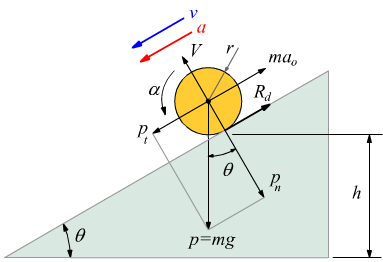
\includegraphics[width = 0.45 \textwidth]{image/motoRototraslatorioPianoIncl.png}
    \caption{Moto rototraslazione di un cilindro pieno su piano inclinato }
    \label{fig:motoRotoTras}
\end{figure}

In questo esercizio, vorremmo capire come è influenzata l'accelerazione di un corpo che rotola giù per un piano inclinato.
Per arrivare alla soluzione del problema dobbiamo utilizzare la legge fondamentale della dinamica rotazionale \ref{equazioneFondamentaleDinamicaRotazionale}.

\begin{equation*}
    M = I\alpha
\end{equation*}

L'equazione rotatoria del cilindro, o disco, pieno è conveniente scriverla rispetto al punto fermo di rotazione \footnote{punto di appoggio del cilindro sul piano inclinato}, e non rispetto al suo baricentro, perché il cilindro sta ruotando rispetto al punto fermo e non rispetto al mozzo il quale si muove durante il rotolamento del cilindro.

Questo punto fermo, ovvero dove avviene la rotazione, è chiamato punto di \textit{istantanea rotazione}.

Il punto di istantanea rotazione continua a cambiare istantaneamente, perché se ruotasse attorno a quel punto dovrebbe entrare nel piano inclinato.

\paragraph{}
La velocità nel punto di istantanea rotazione è:
\begin{equation*}
    V_i = \omega r = \omega * 0  = 0
\end{equation*}

La velocità del baricentro:
\begin{equation*}
    V_b = \omega r
\end{equation*}

Mentre la velocità nel punto più veloce\footnote{diametralmente opposto al punto fermo e viaggia ad una velocità doppia rispetto alla velocità del baricentro} è:
\begin{equation*}
    V_a = 2\omega r = 2V_b
\end{equation*}

Inoltre non mi conviene scrivere l'equazione rispetto al baricentro perché dovrei scrivere il momento di tutte le forze applicate nel baricentro del cilindro: 

\begin{itemize}
    \item la forza peso, però essendo applicato proprio nel baricentro essa ha momento nullo,
    \item la forza normale, $V$,
    \item la forza di attrito, $R_d$,  che agisce sulla ruota ed è proprio questa la forza responsabile del rotolamento.
\end{itemize}

Dopo aver stabilito che non è conveniente scrivere l'equazione rispetto al baricentro, ritorniamo sui nostri passi e iniziamo a scrivere l'equazione rispetto al punto di istantanea rotazione.
I momenti della forze applicate a questo punto sono: 

\begin{itemize}
    \item la forza normale, $V$, è nulla perché il suo momento è zero essendo applicato al punto fermo,
    \item la forza di attrito, $R_d$, come la forza normale, è nulla perché il suo momento è zero essendo applicata al punto fermo,
    \item la forza peso, ed è l'unica che genera momento nel punto di istantanea.
\end{itemize}

Dunque il momento meccanico della forza peso rispetto al punto di rotazione ($M = \vec{r}\times \vec{F}$, braccio prodotto vettoriale forza applicata) è:
\begin{equation*}
   M = \vec{r} \times m\vec{g} = r\sin\theta mg
\end{equation*}

Momento di inerzia rispetto al punto di rotazione, dato dalle principali formule dei momenti di inerzia è la seguente:
\begin{equation*}
   \frac{3}{2}Mr^2
\end{equation*}

\subsubsection{Teorema di Huygens-Steiner }
Per ricavare questo momento di inerzia, oltre che con i valori tabulati dei principali momenti di inerzia, si può applicare il teorema di Huygens-Steiner.

Il teorema afferma che: il momento di inerzia rispetto ad un punto di rotazione, è uguale al momento di inerzia nel baricentro più la massa $M$ per la distanza al quadrato rispetto al punto della rotazione dal baricentro, che in questo caso corrisponde al raggio al quadrato.

\begin{equation*}
   I_0 = \frac{1}{2}MR^2 + MR^2 = \frac{3}{2}MR^2
\end{equation*}

e vediamo che corrisponde al valore della Formula \ref{discoAsseBordo}

\paragraph{}
Accelerazione del momento angolare $\alpha$:\\
l'ultimo ingrediente che ci serve per utilizzare la legge fondamentale, $M = I\alpha$, è calcolare l'accelerazione del momento angolare:

\begin{equation*}
   \alpha = \frac{a_b}{r}\footnote{$a_b$ = accelerazione del baricentro}
\end{equation*}

per trovare l'accelerazione del baricentro basta derivare della velocità del baricentro, $v_b$:

\begin{equation*}
   v_b = \omega r
\end{equation*}
\begin{equation*}
   a_b = \alpha r
\end{equation*}


Ora possiamo scrivere l'equazione del cilindro in discesa sul piano inclinato grazie alla legge fondamentale della dinamica rotazionale \ref{equazioneFondamentaleDinamicaRotazionale}:

\begin{equation*}
    r\sin\theta mg = \frac{3}{2}mr^2\frac{a_b}{r}
\end{equation*}
\begin{equation}
    mg\sin\theta  = \frac{3}{2}mra_b
\end{equation}

dunque l'accelerazione del baricentro è:

\begin{equation*}
    a_b = \frac{2}{3}\biggl(\frac{mg\sin\theta}{m}\biggl)
\end{equation*}
\begin{equation}
    a_b = \frac{2}{3}g\sin\theta
\end{equation}

In questa formula sono da notare due cose: 

\begin{itemize}
    \item $\frac{2}{3}$, tale numero indica che sta rotolando più lentamente, per colpa dell'attrito il quale in questo esempio non lavora ma modifica l'accelerazione, di $\frac{2}{3}$ della accelerazione rispetto ad un oggetto che scivola senza attrito.
    \item la massa non influenza l'accelerazione, infatti si semplifica.
\end{itemize}

Se volessimo trovare il tempo o la velocità finale possiamo utilizzare la formula del moto rettilinea uniformemente accelerato infatti la formula \ref{img:motorettuniformementeacc} diventa:

\begin{equation}
    \frac{h}{\sin{\theta}} = \frac{1}{2}\frac{2}{3}g\sin{\theta}t^2
\end{equation}

dunque il tempo impiegato per scendere è:
\begin{equation}
    t = \sqrt{\frac{3h}{g\sin{\theta}^2}}
\end{equation}

la velocità finale:
\begin{equation}
   v_f = \sqrt{\frac{4}{3}gh} < \sqrt{2gh}\footnote{velocità finale di un corpo che scivola senza attrito}
\end{equation}

\subsubsection{}
Se fosse una sfera piena, il suo momento d'inerzia baricentrale sarebbe:
\begin{equation*}
    I = \frac{2}{5}MR^2
\end{equation*}

applicando il teorema di Huygens-Steiner:
\begin{equation*}
    I = \frac{2}{5}Mr^2 + Mr^2 = \frac{7}{5}Mr^2
\end{equation*}

e dunque l'accelerazione della sfera che scende da un piano inclinato è:
\begin{equation*}
   r\sin\theta mg = \frac{7}{5}mr^2\frac{a_b}{r}
\end{equation*}
\begin{equation}
   a_b = \frac{5}{7}(g\sin\theta)
\end{equation}

Come notiamo la sfera piena avrà un'accelerazione inferiore rispetto ad un oggetto che pattina sul piano inclinato, ma la sua accelerazione è superiore rispetto al cilindro pieno, e questo, di fatto, sta a significare che una biglia su un piano inclinato arriverà prima del cilindro alla base. Di fatto però la biglia si fermerà prima rispetto al cilindro quando inizieranno a viaggiare su un piano piatto.

Questo è dovuto al fatto che il cilindro è più inerte \footnote{cerca di mantenere il suo moto rettilineo uniforme, ovvero la sua velocità} rispetto ad una sfera la quale è più efficiente dal punto di vista inerziale\footnote{si impiega meno forza per partire} del disco. Ciò e dato dal fatto che la massa è più concentrata nel baricentro, mentre nel disco è distribuita in maniera più uniforme.
\paragraph{}
Dato questo paragone si può intuire che un cilindro cavo impiegherebbe ancora più tempo per arriverebbe alla base del piano inclinato, infatti esso minimizza l'accelerazione perché svolgendo i calcoli si avrà la metà, $\frac{1}{2}$, dell'accelerazione di un oggetto che pattina senza attrito.

\subsection{Assi principali di inerzia}

\begin{figure}[H]
    \centering
    \begin{minipage}[c]{0.4\textwidth}
    \centering
    \def\ang{-20}
    \begin{tikzpicture}[rotate=\ang, scale = 1]
      \def\h{0.9}   % length z axis
      \def\L{3.0}   % length rod
      \def\R{1.9}   % circle radius
      \def\r{1.4}   % mass radius (inner sep)
      \coordinate (O) at (0,0);
      \coordinate (L) at (-\R/2,0);
      \coordinate (R) at ( \R/2,0);
      \draw[->](0.18,-\h) -- (-0.465,\h) coordinate (T);
      \pic[xscale=1] at (-0.4,0.7*\h) {rotarr};
      \node[below=1,right=1] at (W3) {$\omega$};
      \draw[line width=1.8,red!25!black] (L) -- (R);
      \node[mass,circle,inner sep=\r,scale=0.8] (L') at (L) {$m_1$};
      \node[mass,circle,inner sep=\r,scale=0.8] (R') at (R) {$m_2$};
      \draw[<->] (L)++(0,-0.2*\R) --++ ( \R/2,0) node[midway,below=-1] {$r_1$}; %\frac{r}{2}
      \draw[<->] (R)++(0,-0.2*\R) --++ (-\R/2,0) node[midway,below=-1] {$r_2$};
      
      \draw[->,myblue](\R/2,0) -- (\R/2,1) node[above,right]{$\vec{l_2}$};
      \draw[->,myblue](-\R/2,0) -- (-\R/2,1) node[above,left]{$\vec{l_1}$};
      \draw[->,myblue](-0.18,0) -- (-0.18,2) node[above,left]{$\vec{L}$};
    
    
    \end{tikzpicture}
    \caption{$\vec{L}$ non proporzionale a $\vec{\omega}$}
    \label{fig:nonProporzionale}
    \end{minipage}
    \hspace{0.1mm}
    \begin{minipage}[c]{0.4\textwidth}
    \centering
    \begin{tikzpicture}[scale = 1]
      \def\h{0.9}   % length z axis
      \def\L{3.0}   % length rod
      \def\R{1.9}   % circle radius
      \def\r{1.4}   % mass radius (inner sep)
      \coordinate (O) at (0,0);
      \coordinate (L) at (-\R/2,0);
      \coordinate (R) at ( \R/2,0);
      \draw[->] (0,-\h) -- (0,\h) coordinate (T);
      \pic[xscale=1] at (0,0.7*\h) {rotarr};
      \node[below=1,right=1] at (W3) {$\omega$};
      \draw[line width=1.8,red!25!black] (L) -- (R);
      \node[mass,circle,inner sep=\r,scale=0.8] (L') at (L) {$m$};
      \node[mass,circle,inner sep=\r,scale=0.8] (R') at (R) {$m$};
      \draw[<->] (L)++(0,-0.2*\R) --++ ( \R/2,0) node[midway,below=-1] {$r$}; %\frac{r}{2}
      \draw[<->] (R)++(0,-0.2*\R) --++ (-\R/2,0) node[midway,below=-1] {$r$};
      
      \draw[->,myblue](\R/2,0) -- (\R/2,1) node[above,right]{$\vec{l_2}$};
      \draw[->,myblue](-\R/2,0) -- (-\R/2,1) node[above,left]{$\vec{l_1}$};
      \draw[->,myblue](0,0) -- (0,2) node[above,left]{$\vec{L}$};
    \end{tikzpicture}
    \caption{Caso simmetria rispetto a $\vec{\omega}$}
    \label{fig:casoSimmetrico}
    \end{minipage}
\end{figure}

Il momento d'inerzia è un vettore che sembra proporzionale al vettore velocità angolare, in realtà vedremo che non è così.
Si prenda come esempio la Figura \ref{fig:nonProporzionale}.

In generale la relazione:

\begin{equation*}
    \vec{L} \neq I\vec{\omega}
\end{equation*}


Calcoliamo il momento angolare di 2 masse puntiformi, e per calcolarlo, basta sommare tutti i momenti angolari: $\vec{r}\times\vec{p}\,\footnote{$\vec{p} = mv$}$.

Si nota ad occhio che il momento angolare totale non è proporzionale rispetto a $\omega$, infatti $I$ non è un semplice scalare ma è un tensore il quale trasforma il vettore $\vec{\omega}$ in un nuovo vettore: $\vec{L}$.
In questo caso $\vec{L}$ è diverso sia in modulo, in direzione e verso rispetto ad $\vec{\omega}$.
\paragraph{}

In figura \ref{fig:casoSimmetrico} viene rappresentatala un caso simile ma con molte simmetrie. In questo caso la relazione $\vec{L} = I\vec{\omega}$ vale in quanto cambia solo il modulo.
Ma momento inerziale intermedio dei tre principali è instabile.


\newpage
\subsection{Conservazione dell'energia meccanica del moto rototraslatorio}
La formula della conservazione dell'energia è ancora valida, ma bisogna aggiungere anche il moto rotatorio perché difatti è energia cinetica, ed è data dalla seguente formula:

\begin{equation*}
    E_{tot} = E_p + E_c
\end{equation*}

\begin{equation}
    E_{tot} = mgh + \frac{1}{2}mv_b^2 + \frac{1}{2}I_b\omega^2
\end{equation}

Riprendendo l'esercizio del piano inclinato svolto a Pagina \pageref{fig:motoRotoTras} possiamo calcolare la velocità finale anche grazie all'energia. Vediamo come:

Sappiamo che l'energia potenziale alla sommità del piano inclinato deve essere uguale all'energia cinetica alla base del piano inclinato $E_p + 0 = 0 + E_c$:
\begin{equation*}
    mgh =  \frac{1}{2}mv_b^2 + \frac{1}{2}I_b\omega^2 = \frac{1}{2}mv_b^2 + \frac{1}{4}mv_b^2 = \frac{3}{4}mv_b^2
\end{equation*}

Dunque la velocità finale è:
\begin{equation}
    v_b = \sqrt{\frac{4}{3}gh}
\end{equation}

che è uguale, ovviamente, a quella trovata con il moto rettilineo uniformemente accelerato.

Più in generale la velocità finale di un corpo che rotola giù su un piano inclinato è la seguente:

\begin{equation}
    v_f = \sqrt{\frac{2gh}{1+\frac{I}{mr^2}}}
\end{equation}

Notiamo che il modulo della velocità dipende dal momento di inerzia e che un momento di inerzia maggiore comporta una velocità minore. 

\subsection{Conservazione del momento angolare}
Il principio di conservazione del momento angolare stabilisce che, se la somma dei momenti delle forze esterne agenti su un corpo è nulla, allora il momento angolare si conserva e quindi costante. 

\begin{equation*}
    \sum \vec{M}_{est} = \sum \frac{\Delta \vec{L}}{\Delta t}
\end{equation*}
dove $\vec{M}_{est}$ e $\vec{L}$ sono definiti nello stesso punto 
\begin{equation*}
    \Delta t\vec{M}_{est} = \Delta\vec{L}
\end{equation*}

ma se $\vec{M_{est}} = 0 $ allora:
\begin{equation*}
    \Delta\vec{L} =  \vec{L}_f -  \vec{L}_i
\end{equation*}

e dunque:
\begin{equation}
   \sum \vec{M}_{est} = 0 \rightarrow  \vec{L}_i = \vec{L}_f 
\end{equation}

Questa legge è l’equivalente rotazionale del principio di conservazione della quantità di moto. 

\paragraph{}
\e possibile estendere il discorso per un sistema di punti: i momenti delle forze interne si elidono a vicenda, per il terzo principio della dinamica, dunque il momento delle forze è dato solo dalla somma dei momenti meccanici esterni. 
Dunque il momento angolare totale si conserva se, come prima, $\sum \vec{M}_{est}  = 0$:

\begin{equation}
    \sum \vec{M}_{est}  = 0 \rightarrow \vec{L}_{tot,i} = \vec{L}_{tot,f}
\end{equation}

\section{La forza di Coriolis}
Nei sistemi di riferimento rotanti può comparire un’altra forza apparente: la forza di Coriolis, dal nome dello scienziato francese che la studiò nel XIX secolo. 
Questa forza:

\begin{itemize}
    \item agisce sugli oggetti in moto rispetto al sistema rotante,
    \item è perpendicolare alla velocità dell’oggetto e all’asse di rotazione.
\end{itemize}

Un oggetto libero, che rispetto a un sistema di riferimento inerziale si muove di moto rettilineo uniforme, Figura \ref{fig:sistemaInerziale}, rispetto a un sistema rotante descrive una traiettoria curvilinea, Figura \ref{fig:sistemaNonInerziale}, a causa della forza di Coriolis.

La forza di Coriolis è direttamente proporzionale alla velocità dell’oggetto e fa deviare
l'oggetto verso destra se il sistema di riferimento ruota in senso antiorario, verso sinistra se il sistema ruota in senso orario.

\def\ang{-20}
\def\R{2}       % disk radius
\def\r{0.1}     % mass radius
\def\v{0.35*\R} % mass velocity
\def\x{0.48}    % mass position (fraction of \R)
\def\ang{50}    % angle displacement
\begin{figure}[H]
    \centering
    \begin{minipage}[c]{0.4\textwidth}
    \centering
    \begin{tikzpicture}
      \coordinate (O) at (0,0);
      \coordinate (T) at (0,\r);
      \coordinate (M) at (90:0.45*\R);
      \coordinate (S) at (-145:1.6*\R);
      \coordinate (B) at (90+\x*\ang:0.88*\R);
      
      % DISK & DOTS
      \draw[disk] (O) circle(\R);
      \fill[myred!20] (90:0.88*\R) circle(0.05*\R);
      \fill[myred] (90+\x*\ang:0.88*\R) circle(0.05*\R);
      \fill[myred!20] (90+\ang:0.88*\R) circle(0.05*\R);
      \draw[xcol,->] (92:0.88*\R) arc(92:88+\ang:0.88*\R);
      
      % MASS
      \draw[<->,black!25,line width=0.9]
        (0,0.35*\R) |-++ (0.35*\R,-0.35*\R);
      \draw[xcol] (O) --++ (90:1.1*\R);
      \draw[vvec] (M) --++ (90:\v) node[below right] {$\vb{v}$};
      \draw[mass] (M) circle(\r) node[right=1] {$m$};
      \draw[->] (10:1.1*\R) arc(10:35:1.1*\R) node[left=2,above=0] {$\omega$};
      
      % AXIS
      \node[left=2] at (S) {S};
      \draw[<->,line width=0.9]
        (S)++(0,0.38*\R) node[left,scale=0.9] {$y$} |-++
             (0.35*\R,-0.35*\R) node[below right=-3,scale=0.9] {$x$};
      
      % AXIS S'
      \draw[<->,line width=0.9]
        (90+\x*\ang:0.35*\R) node[below left=-2,scale=0.9] {$y'$} -- (0,0) --
        (\x*\ang:0.35*\R) node[above=3,right=-2,scale=0.9] {$x'$};
      \node[below=1] at (O) {A};
      \node[right=1,below=1] at (B) {B};
    \end{tikzpicture}
    \caption{Sistema inerziale}
    \label{fig:sistemaInerziale}
    \end{minipage}
    \hspace{5mm}
    \begin{minipage}[c]{0.4\textwidth}
    \centering
    \begin{tikzpicture}
      \def\v{0.40*\R}        % mass velocity
      \def\vv{2.0}           % velocity for plot
      \def\FC{0.30*\R}       % Coriolis force
      \def\om{180/pi}        % angular frequency omega
      \def\tmax{1.10}        % maximum t
      \def\xt{0.98*\x*\tmax} % mass position
      \coordinate (T) at (0,\r);
      \coordinate (S) at (-145-\ang:1.6*\R);
      \coordinate (M) at ({\vv*\xt*sin(\om*\xt)},{\vv*\xt*cos(\om*\xt)});
      \coordinate (V) at ({\v*sin(\om*\xt)+\v*\xt*cos(\om*\xt)},{\v*cos(\om*\xt)-\v*\xt*sin(\om*\xt)});
      \coordinate (F) at ({\FC*cos(\om*\xt)-\FC*\xt*sin(\om*\xt)},{-\FC*sin(\om*\xt)-\FC*\xt*cos(\om*\xt)});
      
      % DISK & DOTS
      \draw[disk] (0,0) circle(\R);
      \fill[myred] (90:0.88*\R) circle(0.05*\R);
      
      % AXIS
      \draw[xcol,dashed] (0,0) --++ (90:1.1*\R);
      \node[below left=-1] at (0,0) {S$'$};
      \draw[<->,line width=0.9]
        (0,0.35*\R) node[left,scale=0.9] {$y'$} |-++
        (0.35*\R,-0.35*\R) node[below right=-3.5,scale=0.9] {$x'$};
      
      % MASS
      \draw[xcol,samples=50,smooth,variable=\t,domain=0:\tmax]
        plot({\vv*\t*sin(\om*\t)},{\vv*\t*cos(\om*\t)});
      %\fill[myred] (90-\ang:0.88*\R) circle(0.05); % check
      \draw[vvec] (M) --++ (V) node[above=3,left=0] {$\vb{v}$};
      \draw[force] (M) --++ (F) node[right=-1] {$\vb{F}_\mathrm{Cor}$};
      \draw[mass] (M) circle(\r) node[left=4,above=2] {$m$};
      
      % AXIS
      \node[left=2] at (S) {S};
      \draw[<->,black!25,line width=0.9]
        (-145:1.6*\R)++(0,0.38*\R) node[left,scale=0.9] {$y$} |-++
                       (0.35*\R,-0.35*\R) node[below right=-3,scale=0.9] {$x$};
      \draw[<->,line width=0.9]
        (S)++(90-\ang:0.38*\R) node[left=3,scale=0.9] {$y$} --++ (-90-\ang:0.38*\R) --++
             (-\ang:0.38*\R) node[below right=-3,scale=0.9] {$x$};
      \draw[->] (-165:1.55*\R) arc(-150:-210:0.6*\R) node[midway,left=0] {$\omega$};
      
    \end{tikzpicture}
    \caption{Sistema non inerziale}
    \label{fig:sistemaNonInerziale}
    \end{minipage}
\end{figure} 

\paragraph{}
La forza di Coriolis è anche responsabile di vari fenomeni che avvengono su scala planetaria e che riguardano il movimento delle masse d’aria e delle correnti oceaniche.
\paragraph{}
A causa del suo moto di rotazione e di rivoluzione, come abbiamo visto, la Terra non è un sistema di riferimento inerziale; tuttavia, poiché le accelerazioni centripete legate a questi moti sono centinaia di volte più piccole dell'accelerazione di gravità, nella maggior parte dei casi gli effetti di non inerzialità sono ininfluenti ed è possibile considerare, con ottima approssimazione, un laboratorio terrestre come un sistema di riferimento inerziale. 

Ci sono però delle situazioni in cui le conseguenze del moto di rotazione della Terra e delle forze apparenti da esso generate sono avvertibili. La forza di Coriolis in particolare, fa sì che un oggetto che si muove verso nord sulla superficie terrestre venga deviato verso est o verso ovest, a seconda che si trovi nell'emisfero boreale o nell'emisfero australe, come mostrato in Figura \ref{fig:coriolisTerra}.

\begin{figure}[tb]
    \centering
    \contourlength{0.7pt}
    \begin{tikzpicture}[scale = 1.5]
      \def\E{1.2}
      \coordinate (O) at (0,0);
      
      % EARTH
      \draw[dashed,rotate=-11] (0,-1.3*\E) -- (0,1.45*\E);
      \fill[blue!70!black!70] (0,0) circle (1.2);
      \draw[very thin,ball color=blue!70!black!40,fill opacity=0.2] (0,0) circle (\E);
      \begin{scope}[rotate=-11]
        \draw[-{Latex[length=3,width=2,flex'=1]}] (0,1.22*\E)++(120:{0.2*\E} and 0.1*\E) arc(120:430:{0.2*\E} and 0.1*\E);
        \clip (0,0) circle (\E);
        \fill[white] (0,\E) ellipse ({0.6*\E} and {0.15*\E});
        \fill[white] (0,-\E) ellipse ({0.8*\E} and {0.08*\E});
        \fill[green!70!black!60,rotate=-30] (160:1.1*\E) ellipse ({0.2*\E} and {0.8*\E});
        \fill[green!70!black!60,rotate=40] (-10:1.14*\E) ellipse ({0.2*\E} and {0.9*\E});
        \fill[green!60!black!60,very thick,rotate=-20] % Australia
          (230:0.86*\E) ellipse ({0.25*\E} and {0.18*\E});
        \draw[dashed] (-\E,0) to[out=-20,in=-160] (\E,0);
        
        % CORIOLIS
        \draw[myred,mydashed,very thin] (0,-0.1*\E) coordinate (NS) --++ (0, 0.70*\E) coordinate (NN);
        \draw[myred,mydashed,very thin] (0,-0.3*\E) coordinate (SN) --++ (0,-0.60*\E) coordinate (SS);
        \draw[myred,mydashed,very thin] (-0.4*\E,0.32*\E) coordinate (NW) to[out=-20,in=-160]++ (0.8*\E,0) coordinate (NE);
        \draw[myred,mydashed,very thin] (-0.4*\E,-0.53*\E) coordinate (SW) to[out=-20,in=-160]++ (0.8*\E,0) coordinate (SE);
        \draw[myarr,red] (NN) to[out=-90,in=  50]++ (-110:0.35*\E); % northern hemisphere
        \draw[myarr,red] (NS) to[out= 90,in=-120]++ (  70:0.35*\E);
        \draw[myarr,red] (SN) to[out=-90,in= 130]++ ( -65:0.30*\E); % southern hemisphere
        \draw[myarr,red] (SS) to[out= 90,in= -60]++ ( 110:0.30*\E);
        \draw[myarr,red] (NE) to[out=200,in= -40]++ (170:0.38*\E); % northern hemisphere
        \draw[myarr,red] (NW) to[out=-20,in= 140]++ (-30:0.42*\E);
        \draw[myarr,red] (SE) to[out=200,in=  40]++ (210:0.42*\E); % southern hemisphere
        \draw[myarr,red] (SW) to[out=-20,in=-140]++ ( 10:0.38*\E);
      \end{scope}
      
      \node at (108-11:1.2*\E) {N};
      \node at (180-11:1.2*\E) {W};
      \node at (   -11:1.2*\E) {E};
      \node at (-98-11:1.2*\E) {S};
      
    \end{tikzpicture}
    \caption{Forza di Coriolis nei due emisferi}
    \label{fig:coriolisTerra}
\end{figure}